\chapter[Grafos]{Grafos}\label{cap.grafos}

\begin{section}{Grafos y sus representaciones}\label{seccion-grafos}

Los objetos a los cuales llamaremos \textit{grafos} son muy útiles en matemática discreta. Su nombre se deriva del hecho de que pueden ser entendidos con una notación gráfica (o pictórica), y en este aspecto solamente se parecen a los familiares gráficos de funciones que son estudiados en matemática elemental. Pero
nuestros grafos son bastante diferentes de los gráficos de funciones y están más relacionados con objetos que en el lenguaje diario llamamos \textit{redes} (networks).  \index{redes}

Usaremos la siguiente definición en lo que sigue: dado un conjunto $X$ un \textit{$2$-subconjunto} es un subconjunto de $X$ de dos elementos.  

\begin{definicion} Un \textit{grafo} $G$ consiste de un  \index{grafo} conjunto finito $V$, cuyos miembros son llamados  \textit{vértices},  \index{vértices de un grafo} y un conjunto de $2$-subconjuntos de $V$, cuyos miembros son llamados \textit{aristas}.  \index{aristas de un grafo} Nosotros usualmente escribiremos $G=(V,E)$ y diremos que $V$ es el \textit{conjunto de vértices} y $E$ es el \textit{conjunto de aristas}.
\end{definicion}

La restricción a un conjunto finito no es esencial, pero es conveniente para nosotros debido a que no consideraremos ``grafos infinitos'' en este apunte.

Un ejemplo típico de un grafo $G=(V,E)$ es dado por los conjuntos
\begin{equation}\label{grafosimple}
V=\{a,b,c,d,z\}, \qquad\quad
E=\{\{a,b\},\{a,d\},\{b,z\},\{c,d\},\{d,z\}\}.
\end{equation}
Este ejemplo y la definición misma no son demasiado esclarecedores, y solamente cuando con\-si\-de\-ra\-mos la \textit{representación pictórica} de un grafo es cuando se hace la luz. \index{representación pictórica (de un grafo)}

\begin{figure}[ht]
    \begin{center}
        \begin{tikzpicture}[scale=1]
        %\SetVertexSimple[Shape=circle,FillColor=white]
        \Vertex[x=0.00, y=2.00]{$a$}
        \Vertex[x=1.90, y=0.62]{$b$}
        \Vertex[x=1.18, y=-1.62]{$c$}
        \Vertex[x=-1.18, y=-1.62]{$d$}
        \Vertex[x=-1.90, y=0.62]{$z$}
        \Edges($c$, $d$,$a$,$b$,$z$,$d$)
        \end{tikzpicture}
    \end{center}    
    \caption{Una representación pictórica del grafo definido en (\ref{grafosimple}).}\label{f5.1}
\end{figure}




Nosotros representamos los vértices como puntos, y unimos dos puntos con una linea siempre y cuando el correspondiente par de vértices está en una arista. Luego la Fig. \ref{f5.1} es una representación pictórica del grafo dado en el ejemplo arriba. Esta clase de representación es extremadamente conveniente para
trabajar ``a mano'' con grafos relativamente pequeños. Más aún, esta representación es de gran ayuda para formular y comprender argumentos abstractos. 

\begin{definicion}
    La \textit{{valencia}} o \textit{grado} de un vértice $v$ en un grafo $G=(V,E)$ es el \index{valencia de un vértice} número de aristas de $G$ que contienen a $v$. Usaremos la notación $\delta(v)$ para la valencia de $v$, formalmente
$$
\delta(v)=|D_v|, \quad \text{ donde } \quad D_v=\{e \in E| v\in
e\}.
$$
\end{definicion}

Por ejemplo, el grafo descrito en Fig. \ref{f5.1} tiene $\delta(a)=2$, $\delta(b)=2$, $\delta(c)=1$, $\delta(d)=3$, $\delta(z)=2$.



Nosotros damos a continuación un ejemplo frívolo de un problema que se resuelve  pensándolo como un grafo.

\begin{figure}[h]
    \begin{center}
        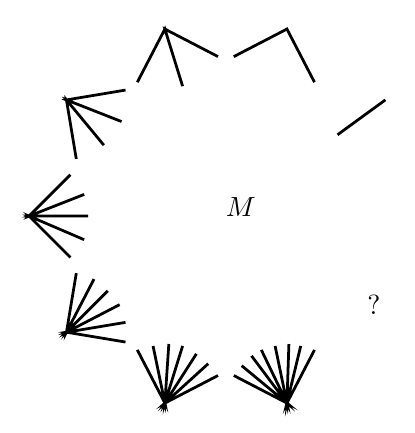
\begin{tikzpicture}[scale=2.5]
        \draw[-,line width=1pt] (0.81,0.59) -- (0.7*0.81,0.7*0.59);
        \draw[-,line width=1pt] (0.31,0.95) -- (0.04, 0.81) -- (0.31,0.95) -- (0.45, 0.68) -- (0.31,0.95);
        \draw[-,line width=1pt] (-0.31,0.95) -- (-0.45, 0.68) -- (-0.31,0.95) -- (-0.22, 0.66) -- (-0.31,0.95) -- (-0.04, 0.81) -- (-0.31,0.95);
        \draw[-,line width=1pt] (-0.81,0.59) -- (-0.76, 0.29) -- (-0.81,0.59) -- (-0.62, 0.36) -- (-0.81,0.59) -- (-0.53, 0.48) -- (-0.81,0.59) -- (-0.51, 0.64) -- (-0.81,0.59);
        \draw[-,line width=1pt] (-1.0,-0.0) -- (-0.79, -0.21) -- (-1.0,-0.0) -- (-0.72, -0.12) -- (-1.0,-0.0) -- (-0.7, -0.0) -- (-1.0,-0.0) -- (-0.72, 0.11) -- (-1.0,-0.0) -- (-0.79, 0.21) -- (-1.0,-0.0);
        \draw[-,line width=1pt] (-0.81,-0.59) -- (-0.51, -0.64) -- (-0.81,-0.59) -- (-0.51, -0.54) -- (-0.81,-0.59) -- (-0.54, -0.45) -- (-0.81,-0.59) -- (-0.6, -0.38) -- (-0.81,-0.59) -- (-0.67, -0.32) -- (-0.81,-0.59) -- (-0.76, -0.29) -- (-0.81,-0.59);
        \draw[-,line width=1pt] (-0.31,-0.95) -- (-0.04, -0.81) -- (-0.31,-0.95) -- (-0.09, -0.75) -- (-0.31,-0.95) -- (-0.15, -0.7) -- (-0.31,-0.95) -- (-0.22, -0.66) -- (-0.31,-0.95) -- (-0.29, -0.65) -- (-0.31,-0.95) -- (-0.37, -0.66) -- (-0.31,-0.95) -- (-0.45, -0.68) -- (-0.31,-0.95);
        \draw[-,line width=1pt] (0.31,-0.95) -- (0.45, -0.68) -- (0.31,-0.95) -- (0.38, -0.66) -- (0.31,-0.95) -- (0.32, -0.65) -- (0.31,-0.95) -- (0.25, -0.66) -- (0.31,-0.95) -- (0.18, -0.68) -- (0.31,-0.95) -- (0.13, -0.71) -- (0.31,-0.95) -- (0.08, -0.76) -- (0.31,-0.95) -- (0.04, -0.81) -- (0.31,-0.95);        
        \GraphInit[vstyle=Welsh]
        \Vertices[]{circle}{0,1,2,3,4,5,6,7,8,$M$}
        \draw (0.6,-0.45) node {?};
        \end{tikzpicture} 
    \end{center}
    \caption{La fiesta de Abril}\label{f5.2}
\end{figure}


\begin{ejemplo*} Mario y su mujer Abril dan una fiesta en la cual hay otras cuatro parejas de casados. Las
parejas, cuando arriban, estrechan la mano a algunas personas, pero, naturalmente, no se estrechan la mano entre marido y mujer. Cuando la fiesta finaliza el profesor pregunta a los otros a cuantas personas han estrechado la mano, recibiendo $9$ respuestas diferentes. ¿Cuántas personas estrecharon la mano de Abril?
\end{ejemplo*}
\begin{proof}[Solución] Construyamos un grafo cuyos vértices son las personas que asisten a la fiesta. Las aristas del grafo son las  $\{x,y\}$ siempre y cuando $x$ e $y$ se hayan estrechado las manos. Puesto que hay nueve personas aparte de Mario, y que una persona puede estrechar a lo sumo a otras $8$ personas, se sigue que las $9$ respuestas diferentes que ha recibido el profesor deben ser $0, 1, 2, 3, 4, 5, 6, 7, 8.$
Denotemos los vértices con estos números y usemos $M$ para Mario. Así obtenemos la representación pictórica de la Fig. \ref{f5.2}

Ahora, el vértice $8$ alcanza a todos los otros vértices excepto uno, el cual debe por lo tanto representar a la esposa de $8$. Este vértice debe ser el $0$ el cual por cierto que no está unido al $8$ (ni ob\-via\-men\-te a ningún otro). Luego $8$ y $0$ son una pareja de casados y $8$ está unido a $1, 2, 3, 4, 5, 6, 7$ y $M$. En particular el $1$ está unido al $8$ y ésta es la única arista que parte del $1$. Por consiguiente $7$ no esta unido al $0$ y al $1$ (únicamente), y la esposa de $7$ debe ser $1$, puesto que $0$ esta casado con $8$. Continuando con este razonamiento vemos que $6$ y $2$, y $5$ y $3$ son parejas de casados. Se sigue entonces que $M$ y $4$ están casados, luego el vértice $4$ representa a Abril, quien estrechó la mano de cuatro personas.
\end{proof}

\begin{ejemplo}\label{ejemplo-grafo-rueda}
Los senderos de un jardín han sido diseñados dándoles forma de \textit{grafo rueda} $W_n$ ($n \ge 2$), cuyos vértices son $V=\{0,1,2,\ldots,n\}$ y sus aristas son
$$
\begin{matrix*}[l]
\{0,1\}, &\{0,2\},&\ldots,&\{0,n-1\}, &\{0,n\},&\quad\text{(los rayos de la rueda)}\\
\{1,2\}, &\{2,3\},&\ldots,&\{n-1,n\},&\{n,1\}.&\quad\text{(el perímetro de la rueda)}
\end{matrix*}
$$
Describir una ruta por los senderos de tal forma que empiece y termine en el vértice $0$ y que pase por cada vértice una sola vez.
\end{ejemplo}
\begin{proof}[Solución]
        Primero  dibujemos el grafo para darnos cuenta de por que se llama ``rueda''. Dibujemos $W_6$. El dibujo nos orienta de como puede ser una ruta: $0,1,2,3,4,5,6,0$. 
        \begin{figure}[h]
            \begin{center}
            \begin{tikzpicture}[scale=0.65]
                %\SetVertexSimple[Shape=circle,FillColor=white,MinSize=8 pt]
                %
                \Vertex[x=0.00, y=0.00]{0}            
                \Vertex[x=3.00, y=0.00]{1}
                \Vertex[x=1.50, y=2.60]{2}
                \Vertex[x=-1.50, y=2.60]{3}
                \Vertex[x=-3.00, y=0.00]{4}
                \Vertex[x=-1.50, y=-2.60]{5}
                \Vertex[x=1.50, y=-2.60]{6}
                \Edges(1,2,3,4,5,6,1)
                \Edges(1,0,4) \Edges(2,0,5) \Edges(3,0,6) 
            \end{tikzpicture}
        \end{center}
        \end{figure}
        

        En  general una respuesta para $W_n$ es: $0,1,2,3,\cdots,n-1,n,0$.   
\end{proof}

Aunque la representación pictórica es intuitivamente atractiva para los seres humanos, es claramente inútil cuando deseamos comunicarnos con una computadora. Para lograr esto debemos re\-pre\-sen\-tar el grafo mediante el conjunto de aristas, como en la definición formal, o cierta clase de lista o tabla. Diremos que dos vértices $x$ e $y$ de un grafo son \textit{adyacentes} cuando $\{x,y\}$ es una arista. \index{vértices adyacentes} (o también diremos que $x$ e $y$ son \textit{vecinos}).  Entonces podemos representar un grafo $G=(V,E)$ por su \textit{lista de adyacencia},  \index{lista de adyacencia} donde cada vértice $v$ encabeza una lista de aquellos vértices que son adyacentes a $v$. El grafo de Fig. \ref{f5.1} tiene la siguiente lista de adyacencia:

\begin{center}
\begin{tabular}{ccccc}
$a$&$b$&$c$&$d$&$z$ \\ \hline
$b$&$a$&$d$&$a$&$b$ \\
$d$&$z$&&$c$&$d$\\
&&&$z$&
\end{tabular}
\end{center}

Las listas de adyacencia son redundantes (cada arista está representada dos veces) pero como todo lenguaje de programación de alto nivel maneja la estructura tipo lista,  preferimos esta representación pues  un grafo  resulta ser una lista de listas  o un  arreglo de listas.  

\begin{observacion*}
    ¿Por qué es más eficiente la representación de un grafo por una lista de adyacencia que por los conjuntos que lo definen?. En  los algoritmos sobre grafos una de las operaciones más utilizadas es encontrar los vértices adyacentes a un vértice dado $v$. En la implementación natural por conjuntos  esto supone recorrer todas las aristas del grafo para determinar en cuales de ellas se encuentra $v$. En un grafo  con gran cantidad de aristas esto supone muchísimas operaciones. En cambio si trabajamos con listas de adyacencia es simplemente devolver la lista correspondiente a $v$ y la cantidad necesaria de operaciones para hacer esto es del orden de la valencia de $v$ (que puede ser un número muy pequeño comparada la número de aristas).   
\end{observacion*}


\begin{definicion}
Por cada entero positivo $n$ definimos el \textit{grafo completo  \index{grafo completo} $K_n$} como el grafo con $n$ vértices y en el cual cada par de vértices es adyacente. 
\end{definicion}


¿Cuántas aristas tiene $K_n$? ¿Cuál es la valencia de cada vértice? De cada vértice ``salen'' $n-1$ aristas, las que van a otros vértices. Luego, cada vértice tiene valencia $n-1$. Si  sumamos $n$-veces las $n-1$ aristas que salen de cada vértice es claro que estamos contando cada arista dos veces, luego el número total de aristas es $n(n-1)/2$ (observar que esta es una demostración, usando  grafos, de que $\sum_{i=1}^n i = n(n-1)/2$).


\subsection*{$\S$ Ejercicios}
\begin{enumex}
\item A tres casas $A,B,C$ se les debe conectar el gas, el agua y la electricidad: $G,W,E$. Escribir la lista de adyacencia para el grafo que representa este problema y construir una representación pictórica del mismo. ¿Puede usted encontrar un dibujo en el cual las líneas que representan las aristas no se crucen?
\item  ¿Para cuales valores de $n$ se puede hacer una representación pictórica
de $K_n$ con la propiedad que las líneas que representan las aristas no se corten? 
\item Un \textit{{$3$-ciclo}} en un grafo es un conjunto de tres vértices mutuamente adyacentes. Construir un grafo con cinco vértices y seis aristas que no contenga $3$-ciclos.
\end{enumex}

\end{section}


\begin{section}{Isomorfismo de grafos} \label{seccion-isomorfismo-de-grafos}
En este punto nosotros debemos enfatizar que un grafo esta definido como una entidad matemática abstracta. Es en este contexto que nosotros discutiremos el importante problema de que queremos decir cuando decimos que dos grafos son ``el mismo''.

Claramente lo importante de un grafo no son los nombres con que designamos a los vértices, ni su representación pictórica o cualquier otra representación. La propiedad característica de un grafo es la manera en que los vértices están conectados por aristas. 

Antes de definir isomorfismo de grafos repasaremos el  concepto de función o aplicación biyectiva. Dado  dos conjuntos $X,Y$ diremos que una aplicación $f: X \to Y$ es \textit{biyectiva} si para cada $y \in Y$ existe un  único $x \in X$ tal que $f(x) =y$. Un propiedad importante, de las funciones biyectivas es que $f$ es biyectiva si y sólo sí  $f$ tiene \textit{inversa}, es decir existe $f^{-1}: Y \to X$, tal que $f(f^{-1}(y)) = y$, $\forall \,y \in Y$ y $f^{-1}(f(x)) = x$, $\forall \,x \in X$.

\begin{ejemplo*}
La función  
\begin{align*}
f&: \{1,2,3\}\to\{a,b,c\} \quad \text{definida } f(1) = c, f(2) = b, f(3) = a
\end{align*}
es biyectiva y su  inversa es 
$$
f^{-1}(a) = 3,\;f^{-1}(b) = 2,\;f^{-1}(c) =1.
$$
También es biyectiva la aplicación
\begin{align*}
g&: \{x,y\}\times \{u,w,z\} \to \{1,2,3,4,5,6\} \quad \text{definida } 
\end{align*}
$$
g(x,u)= 1,\, g(x,w) =2,\, g(x,z) =3,\, g(y,u) =4,\, g(y,w) =5,\, g(y,z) =6. 
$$
\end{ejemplo*}

\begin{definicion} Dos grafos $G_1$ y $G_2$ se dicen que son \textit{isomorfos} cuando  existe una biyección $\alpha$ entre el  \index{grafos isomorfos}  \index{isomorfismo de grafos} conjunto de vértices de $G_1$ y el conjunto de vértices de $G_2$ tal que  si $\{x,y\}$ es una arista de $G_1$ entonces $\{\alpha(x),\alpha(y)\}$ es una arista de $G_2$ y recíprocamente si  $\{z,w\}$ es una arista de $G_2$ entonces $\{\alpha^{-1}(z),\alpha^{-1}(w)\}$ es una arista de $G_1$. La biyección $\alpha$ es llamada un \textit{isomorfismo}.
\end{definicion}

Es importante notar que, debido a al definición, un isomorfismo de grafos se extiende a un biyección de aristas del primer grafo en el segundo grafo. Por lo tanto, para demostrar  que $\alpha$ es un isomorfismo entre dos grafos $G_1$ y $G_2$ alcanza con verificar que lleva en forma inyectiva todas las aristas de $G_1$  en todas las aristas de $G_2$.   

Por ejemplo, considere los dos grafos de la Fig. \ref{f5.3}. En este caso hay una biyección entre el conjunto de vértices de $G_1$ y el conjunto de vértices de $G_2$ la cual tiene la propiedad requerida; esta biyección es dada por
$$
\alpha(a)=t,\quad \alpha(b)=v,\quad \alpha(c)=w,\quad \alpha(d)=u.
$$
Podemos comprobar que a cada arista de $G_1$ le corresponde una arista de $G_2$ y vi\-ce\-ver\-sa. Por ejemplo, a la arista $bc$ de $G_1$ le corresponde la arista $vw$ de $G_2$, y así siguiendo. (Usaremos la abreviación $xy$ para la arista $\{x,y\}$, recordando que una arista es un par desordenado, es decir $xy$ es lo mismo que $yx$.)

\begin{figure}[ht]
    \begin{center}
    \begin{tabular}{llll}
        &
        \begin{tikzpicture}[scale=1]
        %\SetVertexSimple[Shape=circle,FillColor=white]
        \Vertex[x=0,y=0]{$a$}
        \Vertex[x=2,y=0]{$b$}
        \Vertex[x=2,y=-2]{$c$}
        \Vertex[x=0,y=-2]{$d$}
        \Edges($a$, $b$,$c$,$d$,$a$,$b$,$d$)
        \draw (1,-3) node {$G_1$};
        \end{tikzpicture}
        &
        \qquad
        & 
        \begin{tikzpicture}[scale=1]
        %\SetVertexSimple[Shape=circle,FillColor=white]
        \Vertex[x=1,y=0]{$t$}
        \Vertex[x=1,y=-1.3]{$w$}
        \Vertex[x=2,y=-2]{$v$}
        \Vertex[x=0,y=-2]{$u$}
        \Edges($v$, $t$,$u$,$v$,$w$,$u$)
        \draw (1,-3) node {$G_2$};
        \end{tikzpicture}
    \end{tabular}
    \end{center}
    \caption{$G_1$ y $G_2$ son isomorfos} \label{f5.3}
\end{figure}

Cuando, como en la Fig. \ref{f5.3}, dos grafos $G_1$ y $G_2$ son isomorfos usualmente nos referiremos a ellos como que son ``el mismo'' grafo. 

Para mostrar que dos grafos no son isomorfos, nosotros debemos demostrar que no hay una biyección entre el conjunto de vértices de uno con el conjunto de vértices de otro, que lleve las aristas de uno en las aristas del otro.

\begin{figure}[ht]
    \begin{center}
\begin{tabular}{llll}
    &
    \begin{tikzpicture}[scale=1]
    %\SetVertexSimple[Shape=circle,FillColor=white]
    \Vertex[x=0.00, y=2.00]{$a$}
    \Vertex[x=1.90, y=0.62]{$b$}
    \Vertex[x=1.18, y=-1.62]{$c$}
    \Vertex[x=-1.18, y=-1.62]{$d$}
    \Vertex[x=-1.90, y=0.62]{$e$}
    \Edges($c$, $b$,$a$,$e$,$d$,$b$,$a$,$d$)
    \Edges($e$,$b$)
    \draw (0,-2.2) node {$G_1$};
    \end{tikzpicture}
    &
    \qquad
    & 
    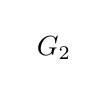
\begin{tikzpicture}[scale=1]
    %\SetVertexSimple[Shape=circle,FillColor=white]
    \Vertex[x=0.00, y=2.00]{1}
    \Vertex[x=1.90, y=0.62]{2}
    \Vertex[x=1.18, y=-1.62]{3}
    \Vertex[x=-1.18, y=-1.62]{4}
    \Vertex[x=-1.90, y=0.62]{5}
    \Edges(1,2,3,4,5,1)
    \Edges(4,2,5)
    \draw (0,-2.2) node {$G_2$};
    \end{tikzpicture}
\end{tabular}
\end{center}
    \caption{$G_1$ y $G_2$ no son isomorfos} \label{f5.4}
\end{figure}

Si dos grafos tienen diferente número de vértices, entonces no es posible ninguna biyección, y los grafos no pueden ser isomorfos. Si los grafos tienen el mismo número de vértices, pero di\-fe\-ren\-te número de aristas, entonces hay biyecciones de vértices  pero ninguna de ellas puede ser un isomorfismo. 

\begin{definicion} 
Sea $G=(V,E)$ un grafo. Se dice que $G^{\prime}=(V^{\prime},E^{\prime})$ es \textit{subgrafo} de
$G=(V,E)$ si $V^{\prime} \subset V$, $E^{\prime} \subset E$ y todos los vértices que son extremos de las aristas de $E^{\prime}$
están en $V^{\prime}$.
\end{definicion}

Es claro, pero  no lo demostraremos aquí, que un isomorfismo lleva un subgrafo a un subgrafo isomorfo. Este resultado es una herramienta que puede ser útil para ver si dos grafos no son isomorfos. 

Por ejemplo, los dos grafos de la Fig. \ref{f5.4} tienen cada uno cinco vértices y siete aristas pero no son isomorfos. Una manera de ver esto es observar que los vértices $a$, $b$, $d$, $e$ forman un subgrafo completo de $G_1$ (cada par de ellos está conectado por una arista). Cualquier isomorfismo debe llevar estos vértices en cuatro vértices de $G_2$ con la misma propiedad, y puesto que no hay tal conjunto de vértices en $G_2$ no puede haber ningún isomorfismo.

\subsection*{$\S$ Ejercicios}\label{ejercicios5.2}
\begin{enumex}
\item Probar que los grafos mostrados en la Fig. \ref{f5.5} no son isomorfos.
\begin{figure}[ht]
    \begin{center}
    \begin{tabular}{llll}
        &
        \begin{tikzpicture}[scale=1]
        \SetVertexSimple[Shape=circle,FillColor=white,MinSize=8 pt]
        \Vertex[x=0.00, y=2.00]{a}
        \Vertex[x=2., y=-1.50]{b}
        \Vertex[x=-2., y=-1.50]{c}
        \Edges(a,b,c,a)
        \Vertex[x=0.00, y=0.85]{1}
        \Vertex[x=1., y=-0.9]{2}
        \Vertex[x=-1., y=-0.9]{3}
        \Edges(1,2,3,1)
        \Edges(a,1,3,c,b,2)
        \draw (0,-2.2) node {$G_1$};
        \end{tikzpicture}
        &
        \qquad
        & 
        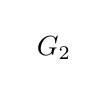
\begin{tikzpicture}[scale=0.65]
        \SetVertexSimple[Shape=circle,FillColor=white,MinSize=8 pt]
        %                
        \Vertex[x=3.00, y=0.00]{1}
        \Vertex[x=1.50, y=2.60]{2}
        \Vertex[x=-1.50, y=2.60]{3}
        \Vertex[x=-3.00, y=0.00]{4}
        \Vertex[x=-1.50, y=-2.60]{5}
        \Vertex[x=1.50, y=-2.60]{6}
        \Edges(1,2,3,4,5,6,1)
        \Edges(1,4) \Edges(3,6) \Edges(2,5)
        \draw (0,-3.8) node {$G_2$};
        \end{tikzpicture}
    \end{tabular}
\end{center}
    \caption{Probar que estos grafos no son isomorfos}\label{f5.5}
\end{figure}

\item \label{ejercicio5.2.2}Encontrar un isomorfismo entre los grafos definidos por las siguientes listas de
adyacencias. Ambas listas especifican versiones de un grafo famoso conocido como \textit{grafo de Petersen}. \index{grafo dePetersen}
$$
\begin{matrix}
a&b&c&d&e&f&g&h&i&j\\ \hline
b&a&b&c&d&a&b&c&d&e\\
e&c&d&e&a&h&i&j&f&g\\
f&g&h&i&j&i&j&f&g&h
\end{matrix}
\qquad \begin{matrix}
0&1&2&3&4&5&6&7&8&9\\ \hline
1&2&3&4&5&0&1&0&2&6\\
5&0&1&2&3&4&4&3&5&7\\
7&6&8&7&6&8&9&9&9&8
\end{matrix}
$$

\item Sea $G=(V,E)$ el grafo definido como sigue: el conjunto de vértices $V$ es el conjunto de todas las palabras de longitud tres en el alfabeto $\{0,1\}$, y el conjunto de aristas $E$ contiene aquellos pares de palabras que difieren exactamente en una posición. Probar que $G$ es isomorfo al grafo formado por las esquinas y aristas de un cubo.
\end{enumex}

\end{section}


\begin{section}{Valencias de un grafo}\label{seccion-valencias-de-un-grafo}
El primer teorema de la teoría de grafos nos dice que la suma de las valencias de un grafo  es dos veces el número de aristas.

\begin{teorema}\label{t5.3} La suma de los valores de las valencias $\delta(v)$, tomados sobre todos los vértices $v$ del grafo $G=(V,E)$, es igual a dos veces el número de aristas:
$$
\sum_{v \in V} \delta(v) = 2|E|.
$$
\end{teorema}
\begin{proof} La valencia de un vértice $v$ indica la cantidad de ``extremos'' de aristas que ``tocan'' a $v$. Es claro que hay $2|E|$ extremos de aristas, luego la suma total de las valencias de los vértices es $2|E|$.
\end{proof}

Hay un útil corolario de este resultado. Diremos que un vértice de $G$ es \textit{impar} si su  \index{vértice impar}  \index{vértice par} valencia es impar, y \textit{par} si su valencia es par. Denotemos $V_i$ y $V_p$ los conjuntos de vértices impares y pares respectivamente, luego $V=V_i \cup V_p$ es una partición de $V$. Por teorema \ref{t5.3}, tenemos que
$$
\sum_{v \in V_i} \delta(v) + \sum_{v \in V_p} \delta(v)= 2|E|.
$$
Ahora cada término en la segunda suma es par, luego esta suma es un número par. Puesto que el lado derecho también es un número par, la primera suma debe ser también par. Pero la suma de números impares solo puede ser par si el número de términos es par. En otra palabras:

\begin{teorema} El número de vértices impares es par.
\end{teorema}

Este resultado es a veces llamado el ``handshaking lemma'' (handshak $=$ estrechar la mano, darse la  \index{handshaking lemma} mano), debido a que se puede interpretar en términos de gente y darse la mano: dado un conjunto de personas, el número de personas que le ha dado la mano a un número impar de miembros del conjunto
es par. 

\begin{observacion*}
    Cuando representamos un grafo por una lista de adyacencia, como cada arista se encuentra dos veces (si $w$ está en la columna de $v$,  entonces $v$  está en la columna de $w$) podemos llegar a pensar que la representación por listas de adyacencia utiliza ``demasiado espacio'' (el doble de lo necesario). Sin embargo,  esta representación ocupa el mismo espacio que la de conjuntos: en la  lista de adyacencia de un grafo $G$, en cada columna $v$  se encuentran $\delta(v)$ vértices. Por lo tanto la tabla tiene $\sum_{v \in V} \delta(v)$  entradas. Por el teorema \ref{t5.3} tenemos que $\sum_{v \in V} \delta(v)= 2|E|$,  es decir el número de entradas de la tabla es dos veces el número de aristas. Por otro lado, como cada arista ocupa $2$ espacios (los dos vértices),  el número de espacios necesario para representar $G$  como conjunto  es también $2|E|$. 
\end{observacion*}

Un grafo en el cual todos los vértices tienen la misma valencia $r$ se llama \textit{regular}  \index{grafo regular} (con valencia $r$), o \textit{$r$-valente,} o de \textit{grado $r$.} En este caso, el de un grafo de grado $r $, el resultado del teorema \ref{t5.3} se traduce a
$$
r|V|=2|E|.
$$

Muchos de los grafos que aparecen en las aplicaciones son regulares. Ya conocemos los  grafos completos $K_n$; ellos son regulares, con valencia $n-1$. De geometría elemental conocemos los polígonos de $n$ lados, los cuales en teoría de grafos son llamados \textit{{grafos cíclicos}}  \index{grafo cíclico} $C_n$. Formalmente, podemos decir que el conjunto de vértices de $C_n$ es $\mathbb Z_n$, y los vértices $i$ y $j$ están unidos si $j=i+1$ o $j=i-1$ en $\mathbb Z_n$. Claramente, $C_n$ es un grafo regular con valencia $2$, si $n\ge 3$.

Una aplicación importante de la noción de valencia es en el problema de determinar si dos grafos son o no isomorfos. Si $\alpha:V_1 \to  V_2$ es un isomorfismo entre $G_1$ y $G_2$, y $\alpha(v)=w$, entonces cada arista que contiene a $v$ se transforma en una arista que contiene a $w$. En consecuencia $\delta(v)=\delta(w)$. Por otro lado, si $G_1$ tiene un vértice $x$, con valencia $\delta(x)=\delta_0$, y $G_2$ no tiene vértices con valencia $\delta_0$, entonces $G_1$ y $G_2$ no pueden ser isomorfos. Esto nos da otra manera para distinguir los grafos de la Fig \ref{f5.4}, puesto que el primer grafo tiene un vértice de valencia 1 y el segundo no.

Una extensión de esta idea se da en la siguiente proposición.

\begin{proposicion}\label{criterioiso}Sean  $G_1$ y $G_2$ grafos isomorfos. Para cada $k\ge 0$ sea $n_i(k)$ el número de vértices de $G_i$ que tienen valencia $k$ ($i=1,2$). Entonces $n_1(k)=n_2(k)$.
\end{proposicion}
\begin{proof} Hemos visto más arriba que si $\alpha:V_1 \to  V_2$ es un isomorfismo entre $G_1$ y $G_2$ y $v\in V_1$, entonces $\delta(v)=\delta(\alpha(v))$. Luego la cantidad de vértices con valencia $k$ en $G_1$ es igual  a la cantidad de vértices con valencia $k$ en $G_2$.     
\end{proof}

\begin{ejemplo*} Revisemos los grafos de la Fig. \ref{f5.4} y la Fig. \ref{f5.5} de la sección anterior.  Los dos grafos de la Fig. \ref{f5.4}  no son isomorfos debido a que en el primer grafo existen tres vértices con valencia $3$ mientras que en el segundo existen sólo dos.

Observar que los criterios vistos hasta ahora relativos a cantidad de vértices,  cantidad de aristas y valencias, incluyendo el de la proposición \ref{criterioiso}, no son útiles para determinar si los grafos de  la Fig. \ref{f5.5} son isomorfos o no: ambos tienen $6$ vértices, $9$ aristas y todos los vértices son de valencia $3$. Sin embargo, en el caso de la Fig. \ref{f5.5} podemos determinar que los grafos no son isomorfos observando los subgrafos de cada uno. Ahora bien, no  hay ningún criterio general eficiente para determinar si dos grafos son isomorfos o no: en los casos difíciles esencialmente debemos probar con todas las biyecciones posibles de los vértices de un grafo a los vértices del otro y eso es no computable para casos no demasiado  grandes.   
\end{ejemplo*}

Ahora veremos el grafo complemento, que, a veces, es una herramienta útil para probar que dos grafos no son isomorfos.

\begin{definicion}
    Si $G=(V,E)$ es un grafo, el \textit{complemento}\index{complemento de un grafo} $G^c$ de $G$ es el grafo cuyo conjunto de vértices es $V$ y cuyas aristas unen aquellos vértices que no son unidos por $G$. 
\end{definicion}

Si $G$ es  un grafo de $n$ vértices,  el complemento de $G$ también puede verse como el grafo  completo $K_n$ ``menos'' $G$. Esto está ejemplificado en la siguiente figura.


\begin{center}
    \begin{tabular}{llllll}
        &
        \begin{tikzpicture}[scale=0.8]
        %\SetVertexSimple[Shape=circle,FillColor=white]
        \Vertex[x=0.00, y=2.00]{$0$}
        \Vertex[x=1.90, y=0.62]{$1$}
        \Vertex[x=1.18, y=-1.62]{$2$}
        \Vertex[x=-1.18, y=-1.62]{$3$}
        \Vertex[x=-1.90, y=0.62]{$4$}
        \Edges($0$, $2$,$1$,$3$,$0$,$4$,$1$)
        \draw (0,-2.2) node {$G$};
        \end{tikzpicture}
        &
        \qquad
        & 
        \begin{tikzpicture}[scale=0.8]
        %\SetVertexSimple[Shape=circle,FillColor=white]
        \Vertex[x=0.00, y=2.00]{$0$}
        \Vertex[x=1.90, y=0.62]{$1$}
        \Vertex[x=1.18, y=-1.62]{$2$}
        \Vertex[x=-1.18, y=-1.62]{$3$}
        \Vertex[x=-1.90, y=0.62]{$4$}
        \Edges($0$, $2$,$1$,$3$,$0$,$4$,$1$)
        \Edges[color=red]($0$,$1$)
        \Edges[color=red]($2$,$3$)
        \Edges[color=red]($2$,$4$)
        \Edges[color=red]($3$,$4$)
        \draw (0,-2.2) node {$K_5$};
        \end{tikzpicture}
        &
        \qquad
        & 
        \begin{tikzpicture}[scale=0.8]
        %\SetVertexSimple[Shape=circle,FillColor=white]
        \Vertex[x=0.00, y=2.00]{$0$}
        \Vertex[x=1.90, y=0.62]{$1$}
        \Vertex[x=1.18, y=-1.62]{$2$}
        \Vertex[x=-1.18, y=-1.62]{$3$}
        \Vertex[x=-1.90, y=0.62]{$4$}
        \Edges[color=red]($0$,$1$)
        \Edges[color=red]($2$,$3$)
        \Edges[color=red]($2$,$4$)
        \Edges[color=red]($3$,$4$)
        \draw (0,-2.2) node {$G^c$};
        \end{tikzpicture}
    \end{tabular}
\end{center}



Debido a que podemos mirar el complemento de un grafo $G$ como las aristas que le faltan para ser completo, si $G$ tiene $n$ vértices y sus valencias son $d_1,d_2,\ldots,d_n$, entonces las valencias de $G^c$ son $n-1-d_1,n-1-d_2,\ldots,n-1-d_n$. En particular, si $G$ es regular de valencia $r$, entonces $G^c$ es regular de valencia $n-1-r$. 

\begin{proposicion}
    Dos grafos $G_1$ y $G_2$  son isomorfos si y solo si $G_1^c$ y $G_2^c$ son isomorfos. 
\end{proposicion}
\begin{proof}
No es difícil ver que si $\alpha:V_1 \to  V_2$ es un isomorfismo entre $G_1$ y $G_2$ entonces $\alpha$ es un isomorfismo entre $G_1^c$ y $G_2^c$. Recíprocamente, si $\alpha:V_1 \to  V_2$ es un isomorfismo entre $G_1^c$ y $G_2^c$, entonces $\alpha$ es un isomorfismo entre $G_1$ y $G_2$.
\end{proof}

\begin{ejemplo}
    Probar que  los siguientes grafos no son isomorfos.
\begin{center}
    \begin{tabular}{llll}
        &
        \begin{tikzpicture}[scale=1]
        %\SetVertexSimple[Shape=circle,FillColor=white]
        \Vertex[x=0.00, y=2.00]{$0$}
        \Vertex[x=1.90, y=0.62]{$1$}
        \Vertex[x=1.18, y=-1.62]{$2$}
        \Vertex[x=-1.18, y=-1.62]{$3$}
        \Vertex[x=-1.90, y=0.62]{$4$}
        \Edges($0$, $2$,$1$,$3$,$0$,$4$,$1$)
        \draw (0,-2.2) node {$G_1$};
        \end{tikzpicture}
        &
        \qquad\quad
        & 
        \begin{tikzpicture}[scale=1]
        %\SetVertexSimple[Shape=circle,FillColor=white]
        \Vertex[x=0.00, y=2.00]{$a$}
        \Vertex[x=1.90, y=0.62]{$b$}
        \Vertex[x=1.18, y=-1.62]{$c$}
        \Vertex[x=-1.18, y=-1.62]{$d$}
        \Vertex[x=-1.90, y=0.62]{$e$}
        \Edges($a$, $b$, $d$, $c$, $a$, $e$, $b$)
        \draw (0,-2.2) node {$G_2$};
        \end{tikzpicture}
    \end{tabular}
\end{center}
\begin{proof}[Solución] 
    Los grafos tienen el mismo número de vértices y aristas, y todos los vértices son de valencia $3$. Luego, la proposición \ref{criterioiso} no nos permite determinar si los grafos no son isomorfos. Sin embargo, observemos que los dos vértices de valencia $1$ de  $G_1^c$ están unidos por una arista,  mientras que esto no ocurre en $G_2^c$. Luego, por la proposición anterior, $G_1$ y $G_2$ no son isomorfos.
    \begin{center}
        \begin{tabular}{llll}
            &
            \begin{tikzpicture}[scale=1]
            %\SetVertexSimple[Shape=circle,FillColor=white]
            \Vertex[x=0.00, y=2.00]{$0$}
            \Vertex[x=1.90, y=0.62]{$1$}
            \Vertex[x=1.18, y=-1.62]{$2$}
            \Vertex[x=-1.18, y=-1.62]{$3$}
            \Vertex[x=-1.90, y=0.62]{$4$}
            \Edges($0$, $1$)
            \Edges($2$,$3$,$4$,$2$)
            \draw (0,-2.2) node {$G_1^c$};
            \end{tikzpicture}
            &
            \qquad\quad
            & 
            \begin{tikzpicture}[scale=1]
            %\SetVertexSimple[Shape=circle,FillColor=white]
            \Vertex[x=0.00, y=2.00]{$a$}
            \Vertex[x=1.90, y=0.62]{$b$}
            \Vertex[x=1.18, y=-1.62]{$c$}
            \Vertex[x=-1.18, y=-1.62]{$d$}
            \Vertex[x=-1.90, y=0.62]{$e$}
            \Edges($a$, $d$, $e$)
            \Edges($b$, $c$, $e$)
            \draw (0,-2.2) node {$G_2^c$};
            \end{tikzpicture}
        \end{tabular}
    \end{center}

\end{proof}
\end{ejemplo} 


\subsection*{$\S$ Ejercicios}\label{ejercicios5.3}
\begin{enumex}
\item ¿Es posible que las siguientes listas sean las valencias de todos los vértices de un grafo? Si así lo fuera, dar una representación pictórica de tal grafo. (Recordar que hay a lo más una arista que una un par de
vértices dados.)
    \begin{enumex}
        \begin{minipage}{0.4\textwidth}
            \item $2,2,2,3.$
        \end{minipage}
        \begin{minipage}{0.4\textwidth}
            \item $1,2,2,3,4.$
        \end{minipage}

        \begin{minipage}{0.4\textwidth}
            \item $2,2,4,4,4.$
        \end{minipage}
        \begin{minipage}{0.4\textwidth}
            \item $1,2,3,4.$
        \end{minipage}
    \end{enumex}


\item Encontrar todos los grafos posibles (no isomorfos) que pueda, que sean regulares, $4$-valentes y con $7$ vértices. [Ayuda: considere el complemento de esos grafos.]



\item Probar que si $G$ es un grafo con al menos dos vértices, entonces $G$ tiene dos vértices con la misma valencia.
\end{enumex}

\end{section}


\begin{section}{Caminos y ciclos}\label{seccion-caminos-y-ciclos}

Frecuentemente usamos grafos como modelos de situaciones prácticas que involucran rutas: los vértices representan ciudades o cruces, y cada arista representa una ruta o cualquier otra forma de comunicación. Las definiciones de esta sección se comprenderán mejor con esta clase de ejemplo en mente.

\begin{definicion}  Una \textit{caminata} en un grafo $G$ es  \index{caminata} una secuencia de vértices
$$
v_1,v_2,\ldots,v_k,
$$
tal que $v_i$ y $v_{i+1}$ son adyacentes ($1 \le i \le k-1$). Si todos los vértices son distintos, una caminata es llamada un \textit{camino}.  \index{camino}

Un \textit{recorrido}\index{recorrido} es una caminata $v_1,v_2,\ldots,v_k$ donde todas las aristas $\{v_i,v_{i+1}\}$ con $1 \le i \le k-1$ son distintas.  

Llamaremos \textit{ciclo} a una caminata \index{ciclo} $v_1,v_2,\ldots,v_{r+1}$  con $r \ge 3$ y cuyos vértices son distintos exceptuando los extremos, es decir que $v_1,v_2,\ldots,v_{r}$ es un camino de al menos tres vértices y $v_1=v_{r+1}$.  A menudo diremos que es un \textit{$r$-ciclo}, o un ciclo de \textit{longitud} $r$ en $G$.  \index{longitud de un ciclo}
\end{definicion}

Es decir, una caminata especifica una ruta en $G$: del primer vértice vamos a uno adyacente, de éste a otro adyacente y así siguiendo. En una caminata podemos visitar cualquier vértice varias veces, y en particular, podemos ir de un vértice $x$ a otro $y$ y luego tomar la dirección contraria y regresar a $x$. En un camino, cada vértice es visitado solo una vez. En un recorrido los vértices pueden ser visitados varias veces pero no se puede pasar por una arista más de una vez. 

Escribamos $x \sim y$ siempre y cuando $x=y$ o $x \ne y$ y los vértices $x$ e $y$ de $G$ puedan ser unidos por un camino en $G$. Hablando en forma rigurosa, esto significa que cuando $x \ne y$  que hay un camino $v_1,v_2,\ldots,v_k$ en $G$ con $x=v_1$ e $y=v_k$. 

\begin{lema} Sea $G$ un grafo y $x$, $y$  vértices distintos. Entonces, $x \sim y$ si  y sólo si $x$ e $y$ pueden ser unidos por una caminata 
\end{lema}
\begin{proof}Es claro que si $x$ e $y$ están unidos por un camino, como  un camino es un caso especial de caminata, $x$ e $y$ están unidos por una caminata.

Veamos que si  $x$ e $y$ están unidos por una caminata, entonces están unidos por un camino. Sea 
$$
x=x_1,x_2,\ldots,x_k=y,
$$
una caminata entre  $x$ e $y$. Si ninguno de los $x_i$ se repite, entonces tenemos un camino y terminado el problema. Si hay repetición, entonces existe $j$ tal que $x_j = x_{j+r}$ con $r >0$, es decir tenemos una caminata
$$
x=x_1,x_2,\ldots,x_j,\ldots,x_{j+r},\ldots, x_k=y,
$$
Como $x_j = x_{j+r}$ podemos eliminar la subcaminata $x_{j+1},\ldots,x_{j+r}$ (un ``bucle'' dentro de la caminata) y nos queda 
$$
x=x_1,x_2,\ldots,x_j,x_{j+r+1},\ldots, x_k=y,
$$
una caminata, más corta,  entre $x$ e $y$. Esto se ejemplifica en la figura \ref{fig-eliminando-bucles}.


Podemos repetir este procedimiento hasta eliminar todos los ``bucles'' y obtener un camino.
\end{proof}

\begin{figure}[ht]
    \begin{center}
        \begin{tikzpicture}[scale=1]
            \SetVertexSimple[Shape=circle,FillColor=white,MinSize=5 pt]
            %
            %\ponertz{-7}{-30}{$x=$}
            \draw (-0.6,0) node {$x = $};                
            \draw (0,0.4) node {$x_1$};
            \Vertex[x=0.00, y=0]{v0}
            \Vertex[x=1, y=0]{v1}
            \draw (1,0.4) node {$x_2$};
            \Vertex[x=3, y=0]{vi}
            \draw (3,0.4) node {$x_j$};
            \Vertex[x=2.5, y=0.5]{vi1}
            \Vertex[x=2.5, y=1]{vi2}
            \Vertex[x=3.5, y=0.5]{vi3}
            \Vertex[x=3.5, y=1]{vi4}
            \Edges(v0,v1)
            \Edges(vi,vi1)
            \Edges(vi1,vi2)
            \draw (2.7,1.3) node {$\scriptstyle\bullet$};
            \draw (2.9,1.5) node {$\scriptstyle\bullet$};
            \draw (3.1,1.5) node {$\scriptstyle\bullet$};
            \draw (3.3,1.3) node {$\scriptstyle\bullet$};
            \draw (2,0) node {$\scriptstyle\bullet$};
            \draw (2.3,0) node {$\scriptstyle\bullet$};
            \Edges(vi3,vi4)
            \Edges(vi3,vi)
            \Vertex[x=5, y=0]{vr1}
            \Vertex[x=6, y=0]{vr}
            \Edges(vr1,vr)
            \draw (6,0.4) node {$x_k$};
            \draw (5,0.4) node {$x_{k-1}$};
            \draw (6.6,0) node {$=y$};
            
            \SetVertexNormal[LineColor=white]
            \Vertex[x=1.8, y=0]{s1}
            \Vertex[x=2.2, y=0]{s2}
            \Edges(v1,s1)
            \Edges(vi,s2)
            \draw (1.7,0) node {$\scriptstyle\bullet$};
            \draw (2,0) node {$\scriptstyle\bullet$};
            \draw (2.3,0) node {$\scriptstyle\bullet$};
            
            \Vertex[x=4.2, y=0]{t1}
            \Vertex[x=3.8, y=0]{t2}
            \Edges(vr1,t1)
            \Edges(vi,t2)
            \draw (3.7,0) node {$\scriptstyle\bullet$};
            \draw (4,0) node {$\scriptstyle\bullet$};
            \draw (4.3,0) node {$\scriptstyle\bullet$};
        \end{tikzpicture}
    \end{center}
    Se transforma en 
    \begin{center}
        \begin{tikzpicture}[scale=1]
            \SetVertexSimple[Shape=circle,FillColor=white,MinSize=5 pt]
            %
            %\ponertz{-7}{-30}{$x=$}
            \draw (-0.6,0) node {$x = $};                
            \draw (0,0.4) node {$x_1$};
            \Vertex[x=0.00, y=0]{v0}
            \Vertex[x=1, y=0]{v1}
            \draw (1,0.4) node {$x_2$};
            \Vertex[x=3, y=0]{vi}
            \draw (3,0.4) node {$x_j$};
            \Edges(v0,v1)
            \Vertex[x=5, y=0]{vr1}
            \Vertex[x=6, y=0]{vr}
            \Edges(vr1,vr)
            \draw (6,0.4) node {$x_k$};
            \draw (5,0.4) node {$x_{k-1}$};
            \draw (6.6,0) node {$=y$};
            
            \SetVertexNormal[LineColor=white]
            \Vertex[x=1.8, y=0]{s1}
            \Vertex[x=2.2, y=0]{s2}
            \Edges(v1,s1)
            \Edges(vi,s2)
            \draw (1.7,0) node {$\scriptstyle\bullet$};
            \draw (2,0) node {$\scriptstyle\bullet$};
            \draw (2.3,0) node {$\scriptstyle\bullet$};
            
            \Vertex[x=4.2, y=0]{t1}
            \Vertex[x=3.8, y=0]{t2}
            \Edges(vr1,t1)
            \Edges(vi,t2)
            \draw (3.7,0) node {$\scriptstyle\bullet$};
            \draw (4,0) node {$\scriptstyle\bullet$};
            \draw (4.3,0) node {$\scriptstyle\bullet$};
        \end{tikzpicture}
    \end{center} 
    \caption{Eliminando ``bucles''  de una caminata} \label{fig-eliminando-bucles}
\end{figure}


\begin{definicion} Diremos que un grafo  $G$ es \textit{conexo} si para cualesquiera dos vértices $x,y$ existe un camino de $x$ a $y$, es decir si  $x \sim y$. 
\end{definicion}

Debido al lema que probamos más arriba, es sencillo verificar la siguientes propiedades: sea $G$ grafo y sean $x,y,z$ vértices de $G$, entonces
\begin{enumerate}[label=\textit{\alph*)}]
\item  $x \sim x$ (reflexividad de $\sim$).
\item  $x \sim y$, entonces $y \sim x$ (simetría de $\sim$).
\item  $x \sim y$,  $y \sim z$, entonces  $x \sim z$ (transitividad  de $\sim$).
\end{enumerate}


En un lenguaje formal, una relación que  cumple las tres propiedades anteriores es llamada una  \textit{relación de equivalencia}\index{relación de equivalencia} del conjunto, en este caso tenemos una relación de equivalencia del conjunto de vértices $V$ de $G$. Como ya vimos en el capítulo \ref{cap.aritmetica_modular}, página  \pageref{relacion-de-equivalencia}, la congruencia módulo es también una relación de equivalencia, y hay muchísimos ejemplos en matemática de estos tipos de relaciones. 

Estas tres propiedades que posee la relación de equivalencia permiten partir a $V$ en conjuntos disjuntos: dos vértices están en el mismo conjunto si ellos pueden ser unidos por un camino, y están en conjuntos diferentes si no podemos encontrar tal camino. llamaremos a estos conjuntos disjuntos las \textit{clases de equivalencia de $\sim$}.\index{clases de equivalencia}

\begin{definicion}Supongamos que $G=(V,E)$ es un grafo y que la partición de $V$ en las clases de equivalencia de $\sim$ es
$$
V= V_1 \cup V_2 \cup \cdots \cup V_r.
$$
Denotemos con $E_i$ ($1\le i \le r$) al subconjunto de $E$ que contiene todas las aristas cuyos finales están en $V_i$. Entonces los grafos $G_i=(V_i,E_i)$ son llamados las \textit{componentes}  \index{componente de un grafo}  \index{grafo conexo} de $G$. Si $G$ tiene solo una componente entonces, claramente, el grafo es {conexo}.
\end{definicion}

\begin{figure}[t]
    \begin{center}
\begin{tikzpicture}[scale=1.1]
\SetVertexSimple[Shape=circle,FillColor=white,MinSize=8 pt]            
\Vertex[x=6, y=-0.5]{1}
\Vertex[x=5.5, y=-2]{2}
\Vertex[x=7, y=-3.5]{3}
\Vertex[x=7, y=-2]{4}
\Vertex[x=11, y=-2]{5}
\Vertex[x=6.50, y=-1.2]{6}
\Vertex[x=6.50, y=-2.5]{7}
\Vertex[x=9.5, y=-0.8]{8}
\Vertex[x=8.5, y=-2.5]{9}
\Vertex[x=10, y=-3.3]{a}
\Edges(5,1,2,4,5,3,2,4,3,5,4)
\Edges(a,8,9,7,6,8,9)
\end{tikzpicture}
\end{center}
\caption{Un grafo con dos componentes} \label{f5.6}
\end{figure}

La terminología casi explica por si misma el significado de estas definiciones. El grafo mostrado en la Fig. \ref{f5.6} tiene dos componentes, y por consiguiente no es conexo. La descomposición de un grafo en componentes es muy útil, puesto que muchas propiedades de los grafos pueden ser establecidas considerando las componentes separadamente. Por esta razón, teoremas acerca de grafos a menudo son probados solo para la clase de grafos conexos.

Cuando un grafo de moderado tamaño es dado por una representación pictórica es bastante fácil determinar si es o no conexo. Sin embargo, cuando un grafo es dado por una lista de adyacencia necesitaremos un algoritmo eficiente para decidir si es o no conexo. 

\begin{figure}[ht]
    \begin{center}
        \begin{tikzpicture}[scale=1]
        %\SetVertexSimple[Shape=circle,FillColor=white]
        \def\rvar{1.2}
        \Vertex[x=0.00, y=-2.00]{$u$}
        \Vertex[x=\rvar*1.90, y=-0.62]{$t$}
        \Vertex[x=\rvar*1.18, y=1.62]{$q$}
        \Vertex[x=-1.18*\rvar, y=1.62]{$p$}
        \Vertex[x=-1.90*\rvar, y=-0.62]{$r$}
        \Vertex[x=0, y=0]{$s$}
        \Edges($u$,$t$,$q$,$p$,$r$,$u$,$s$,$t$,$r$,$s$,$q$,$r$,$p$,$t$,$s$,$u$,$s$,$p$)
        \end{tikzpicture}
    \end{center}
    \caption{El gran tour} \label{f5.7}
\end{figure}

\subsection*{Ciclos hamiltonianos, caminatas eulerianas}

\begin{ejemplo}\label{chunner} Leandro y Juan, dos amigos, planean tomar sus vacaciones en determinada isla. La Fig. \ref{f5.7} representa los lugares de interés turístico de la isla y las carreteras que los unen. Leandro es un turista por naturaleza, y desea visitar cada lugar una vez y volver al punto de partida. Juan es un explorador, y desea atravesar todos los caminos solo una vez, a él lo tiene sin cuidado si regresa o no al lugar del cual partió. ¿Podrán encontrar las rutas que desean Leandro y Juan?
\begin{proof}[Solución] Leandro puede usar diferentes rutas para alcanzar su objetivo: una posibilidad es el ciclo $p,q,t,s,u,r,p$.
    
    Sin embargo, Juan está en un apuro. Llamemos $x$ al punto de partida y llamemos $y$ al punto de llegada, y supongamos por el momento que $x \not= y$. Entonces él usa una arista con extremo en $x$ para partir y cada vez que vuelve a $x$ debe arribar y partir por nuevas aristas. Luego, usa un número impar de aristas con extremo en $x$, y por consiguiente $x$ debe ser un vértice impar. De manera análoga, $y$ debe ser también un vértice impar, puesto que Juan usa dos aristas cada vez que pasa por $y$, y una más al finalizar en $y$. Los restantes vértices deben ser pares, puesto que cada vez que Juan llega a un vértice intermedio parte de nuevo, y por consiguiente usa dos aristas.
    
    Resumiendo, una ruta para Juan que empiece y finalice en vértices distintos $x$ e $y$, es solo posible si hay dos vértices impares (que son $x$ e $y$) y el resto de los vértices es par.  Pero en el grafo de la Fig. \ref{f5.7} el valor de las valencias es: $\delta(p)=4$, $\delta(q)=4$, $\delta(r)=5$, $\delta(s)=5$, $\delta(t)=5$, y $\delta(u)=3$. Luego hay demasiados vértices impares, y por lo tanto no existe la ruta que Juan desea. Si permitimos la posibilidad de que $x=y$ , la situación es aún peor, pues en este caso todos los vértices deberían ser pares.
\end{proof}
\end{ejemplo}

En general, la ruta de Leandro es un ciclo que contiene todos los vértices del grafo dado. Tales ciclos fueron estudiados por el matemático irlandés W.R. Hamilton (1805-1865),  \index{Hamilton, W. R.} y en consecuencia un ciclo con esta propiedad es llamado un \textit{ciclo hamiltoniano}. En nuestro ejemplo, fue muy fácil \index{ciclo hamiltoniano} encontrar un ciclo hamiltoniano, pero este fue un caso muy especial y no representativo. Para ciertos grafos, puede ser un problema difícil decidir si un ciclo hamiltoniano existe o no.

Por otro lado, el problema de Juan puede ser fácilmente resuelto. Una caminata que use cada arista de un grafo solo una vez, o equivalentemente un recorrido que use todas las aristas, es llamada una \textit{caminata euleriana}, debido a que Euler \index{caminata euleriana} fue el primero en estudiar estas caminatas y encontró que si $x\not= y$, una condición necesaria para que exista una caminata euleriana que comience en $x$ y finalice en $y$ es que $x$ e $y$ deben ser vértices impares y el resto debe ser par, mientras que si $x=y$ la condición es que todos los vértices deben ser pares. Es decir que una condición necesaria para que exista una caminata euleriana en un grafo $G$
es que $G$ debe tener a lo más dos vértices impares. Más aún, puede probarse que esta condición es también suficiente. Puesto que es sencillo calcular las valencias de los vértices de un grafo, es relativamente sencillo decidir si un grafo tendrá o no una caminata euleriana. 

Resumiendo las definiciones de más arriba:

\begin{definicion}
Un \textit{ciclo hamiltoniano} en un grafo $G$ es un ciclo que contiene a todos los vértices del grafo. Una \textit{caminata euleriana} en un grafo $G$ es un recorrido que usa todas las aristas de $G$. Una caminata euleriana que comienza y termina en un mismo vértice se llama también \textit{circuito euleriano}.
\end{definicion}

\begin{ejemplo*}
    En  el ejemplo \ref{ejemplo-grafo-rueda} vimos que dado $n \in \N$, entonces el grafo rueda $W_n$ tiene ciclos hamiltonianos. Con el resultado del teorema \ref{th-caminata-euleriana} veremos que  el grafo rueda nunca tiene caminatas eulerianas. 
\end{ejemplo*}

El siguiente teorema resume los resultados sobre caminatas eulerianas. La demostración no es demasiada complicada, pero la veremos más adelante.  

\begin{teorema}\label{th-caminata-euleriana} Un grafo conexo con más de un vértice posee una caminata euleriana si y solo si tiene a lo más dos vértices de grado impar. 
\begin{enumerate}
    \item\label{item:dos-vertices-impares} El grafo posee una caminata  euleriana de $v$ a $w$, con $v \not= w$ si y sólo si $v$ y $w$ son los únicos vértices de grado impar.
    impar.
    \item\label{item:todos-los-vertices-pares} El grafo tiene un circuito euleriano si y sólo si todos los vértices tienen grado par.
\end{enumerate}
\end{teorema}

\begin{observacion}\label{obs-par-a-impar}
    El caso de un grafo donde todas las valencias son pares se puede reducir al caso donde hay dos vértices impares: si deseamos una caminata euleriana que empiece y termine en $v$, eliminamos una arista del grafo que contenga a $v$, digamos la arista $\{v,w\}$, con lo cual queda un grafo  con solo dos vértices, $v$ y $w$, de valencia impar. Entonces, aplicamos el caso  \ref{item:dos-vertices-impares}, con lo cual hacemos una caminata euleriana que comienza en $v$ y  termina en  $w$. Terminamos la caminata agregando  la arista $\{v,w\}$. 
\end{observacion}


\begin{observacion}\label{obs-impar-a-par}
    Recíprocamente,  el caso de un grafo  $G$ con dos valencias impares y todas las demás valencias pares  se puede reducir al caso en que todas las valencias son pares. Sean $p$ y $q$ los dos vértices de valencia impar,  agregamos un vértice $e$  al grafo y lo unimos a $p$ y $q$. Así obtenemos un grafo donde todas las valencias son pares. Ahora si tenemos  un circuito euleriano partiendo de $e$, el circuito es de la forma
    \begin{equation*}
        e, p,w_1,\ldots,w_r,q,e, 
    \end{equation*}
    o
    \begin{equation*}
        e, q,v_1,\ldots,v_t,p,e. 
    \end{equation*}
    En  ambos caso eliminando $e$ obtenemos una caminata euleriana. En el primer caso la camina euleriana es
    \begin{equation*}
        p,w_1,\ldots,w_r,q, 
    \end{equation*}
    y en el segundo caso es
    \begin{equation*}
        q,v_1,\ldots,v_t,p. 
    \end{equation*}

\end{observacion}

\subsection*{Algoritmo de Hierholzer}

C. Hierholzer (1840-1871) mostró, poco antes de su muerte, un algoritmo fácilmente implementable para encontrar un circuito euleriano  para cualquier grafo  con vértices de grado  par. El lector interesado puede leer el artículo original \href{https://eudml.org/doc/156599}{Ueber die Möglichkeit, einen Linienzug ohne Wiederholung und ohne Unterbrechung zu umfahren}. Mathematische Annalen volume 6, pp. 30–32 (1873) (en alemán). 

El algoritmo de Hierholzer\index{algoritmo de Hierholzer} fue la primera demostración del teorema \ref{th-caminata-euleriana} para el caso  de grafos con vértices de grado par. 
%Obviamente,  debido a la observación  \ref{obs-impar-a-par}, esto demuestra también el teorema para grafos con dos valencias impares. 
Nosotros veremos aquí una versión del algoritmo de Hierholzer que se aplica tanto a los grafos con todos los vértices de valencia par como, a los que tienen dos vértices de valencia impar. 

Para explicar el algoritmo de Hierholzer nos es útil la siguiente definición:  un \textit{recorrido maximal}  es un recorrido que respetando la condición de no repetir aristas no es posible continuarlo como recorrido desde el último vértice.  

La idea clave del algoritmo de Hierholzer  es la siguiente.

\begin{lema}\label{lema:hierholzer}
    \begin{enumerate}
        \item\label{item:hierholzer_a} En un grafo de valencias pares (conexo o no conexo) todo recorrido maximal termina en el vértice original.
        \item\label{item:hierholzer_b} En  un grafo conexo con dos vértices de valencia impar todo recorrido maximal que parte de un vértice de valencia impar termina en el otro vértice de valencia impar.
    \end{enumerate}
\end{lema}
\begin{proof} \ref{item:hierholzer_a}
    Observar que no es posible quedarse atascado en ningún vértice que no sea  el vértice original, porque el grado par de todos los vértices garantiza que, cuando se ingresa a un vértice distinto al original debe haber una  arista sin usar que nos permite dejarlo. 

    \ref{item:hierholzer_b} Saliendo del vértice original, y razonando en forma análoga a  \ref{item:hierholzer_a}, podemos ver fácilmente que el recorrido maximal termina en el vértice impar que no es el origen. 
\end{proof}


Teniendo en cuenta las consideraciones anteriores podemos plantear el siguiente algoritmo:\index{algoritmo de Hierholzer}

Sea $G$ un grafo conexo con vértices de grado par o con dos vértices de grado impar y los demás vértices de grado par. 

\begin{enumerate}
    \item \textbf{Paso 0.} Elija el vértice inicial $v$. Si $G$  tiene todos sus vértices de grado par,  entonces $v$ puede ser cualquier vértice. Si $G$ tiene dos vértices de grado impar,  entonces $v$ debe ser uno de los vértices de valencia impar.
    \item \textbf{Paso 1.} Haga un recorrido maximal partiendo de $v$. 
    
    \item \textbf{Paso iterativo.} Mientras en el recorrido ya realizado no estén todas las aristas del grafo, realice los pasos siguientes.    
    \begin{itemize}
        \item Sea $u$  un vértice que tenga aristas libres, realice un recorrido maximal que parte de $u$ siguiendo las aristas no utilizadas. 
        \item Inserte en $u$ este recorrido al recorrido  anterior obteniendo un nuevo recorrido (más largo).
        \item  Vuelva a (3). 
    \end{itemize}
\end{enumerate}



Observemos que el recorrido del paso 1 en el caso del grafo con todas las valencias pares, es un recorrido cerrado. En el caso del grafo con dos valencias impares es un recorrido que va de un vértice impar al otro.  
    
En  cualquier de los dos casos,  en el paso 1 el recorrido maximal puede no cubrir todos los vértices y aristas del grafo inicial. Además,  observemos que el subgrafo que se obtiene eliminando las aristas del recorrido tiene todas las valencias pares. 

En  el paso iterativo el subgrafo de las aristas disponibles tiene todos los vértices de valencia par y por lo tanto el recorrido comienza y  termina en el mismo vértice y allí se inserta.

Puesto que suponemos que el grafo original es conexo, repetir el paso iterativo agotará todos las aristas del grafo.

\begin{comment}
El  algoritmo es el siguiente: 
\begin{enumerate}
    \item \textbf{Paso 1.} Elija cualquier vértice  inicial $v$ y haga una caminata  que no repita aristas y  que vuelva al vértice (de $v$ a $v$). 
    
    El recorrido formado de esta manera es un recorrido cerrado, pero puede no cubrir todos los vértices y aristas del grafo inicial.

    \item \textbf{Paso iterativo} Mientras exista un vértice $u$ en la caminata ya realizada, pero que tenga aristas que no formen parte de la caminata, inicie otra caminata desde $u$ hasta $u$ siguiendo las aristas no utilizadas. Luego,  inserte esta  caminata a la caminata  anterior para formar una caminata nueva (más larga).
    
    Observemos que el subgrafo formado por todas las aristas utilizadas despues de cada paso iterativo es un grafo con valencias pares y por lo tanto el subgrafo que obtenemos luego de quitar estas aristas también es par. Esto nos permite hacer caminatas cerradas  por aristas no utilizadas desde cada vértice con aristas no utilizadas.
\end{enumerate}

Puesto que suponemos que el grafo original es conexo, repetir el paso iterativo agotará todos las aristas del grafo.
\end{comment}

\begin{ejemplo*} Dado  el  grafo de de la  Fig. \ref{f5.7.1}, encontremos un circuito euleriano con origen en $u$. 

Debemos primero observar que  debe existir un circuito euleriano, pues $\delta(p)=4$, $\delta(q)=4$, $\delta(r)=4$, $\delta(s)=4$, $\delta(t)=4$, y $\delta(u)=2$,  es decir todos los vértices tienen grado par. 


\begin{figure}[ht]
    \begin{center}
    \begin{tikzpicture}[scale=1]
    %\SetVertexSimple[Shape=circle,FillColor=white]
    \def\rvar{1.2}
    \Vertex[x=0.00, y=-2.00, L=$u$]{$u$} % 3
    \Vertex[x=\rvar*1.90, y=-0.62, L=$t$]{$t$} % 2
    \Vertex[x=\rvar*1.18, y=1.62, L=$q$]{$q$} % 1
    \Vertex[x=-1.18*\rvar, y=1.62, L=$p$]{$p$} % 0
    \Vertex[x=-1.90*\rvar, y=-0.62, L=$r$]{$r$} % 4
    \Vertex[x=0, y=0, L=$s$]{$s$} % 5
    \Edges($u$,$t$,$q$,$p$)
    \Edges($r$,$u$)
    \Edges($s$,$t$)
    \Edges($r$,$s$,$q$,$r$)
    \Edges($p$,$t$,$s$)
    \Edges($s$,$p$,$r$)
    \end{tikzpicture}
    \end{center}
    \caption{El gran tour, de nuevo.} \label{f5.7.1}
\end{figure}

Apliquemos el algoritmo de Hierholzer partiendo  desde $u$. Una caminata posible con origen en $u$ y que vuelva a $u$ es $$u, r, p, q, s, t, u.$$


Ahora elijamos $q$ que es un vértice que pertenece a la caminata pero que tiene aristas que no son parte de la caminata (ver figura \ref{f5.7.1b}). Una caminata que no toca aristas usadas y  que parte de $q$ y regresa a $q$ es $q,t,p,s,r,q$.  
Insertamos en $q$  esta caminata  a la caminata anterior y obtenemos:
$$u, r, p, \mathbf{q,t,p,s,r,q}, s, t, u.$$
(En  negrita la caminata insertada).
\end{ejemplo*}


\begin{figure}[ht]
    \begin{center}
    \begin{tikzpicture}[scale=1]
    %\SetVertexSimple[Shape=circle,FillColor=white]
    \def\rvar{1.2}
    \Vertex[x=0.00, y=-2.00, L=$u$]{$u$} % 3
    \Vertex[x=\rvar*1.90, y=-0.62, L=$t$]{$t$} % 2
    \Vertex[x=\rvar*1.18, y=1.62, L=$q$]{$q$} % 1
    \Vertex[x=-1.18*\rvar, y=1.62, L=$p$]{$p$} % 0
    \Vertex[x=-1.90*\rvar, y=-0.62, L=$r$]{$r$} % 4
    \Vertex[x=0, y=0, L=$s$]{$s$} % 5
    \Edges($t$,$q$)
    \Edges($r$,$s$)
    \Edges($q$,$r$)
    \Edges($p$,$t$)
    \Edges($s$,$p$)
    \end{tikzpicture}
    \end{center}
    \caption{El subgrafo de aristas no utilizadas.} \label{f5.7.1b}
\end{figure}

\begin{comment}
\begin{observacion*} Escribiremos en pseudocódigo el algoritmo para hallar una caminata o circuito euleriano en un grafo $G$ con $n$ vértices  de valencia par.
    
Como ya mencionamos anteriormente, a un grafo $G$ lo representaremos por una lista de adyacencia. Supongamos que los vértices de $G$ son $0,\ldots,k$,  entonces $G[i] = [i_0,i_1,\ldots]$ serán los vértices adyacentes al vértice $i$. Tomamos como comienzo del recorrido el vértice arbitrario $0$.





\vskip .4cm
{%\centering
\begin{minipage}{0.95\textwidth}
\noindent \textsc{Circuito euleriano}
\vskip .2cm
\begin{small}
\begin{verbatim}
# pre: G grafo con todos los vértices de valencia par 
# post: cuando termina 'circuito' es una lista de vértices que es
#       un circuito euleriano que empieza en 0 (y termina en 0).
circuito = [0]  # inicio de la caminata
libres = G # aristas no utilizadas
while nº de aristas(libres) > 0:
    sub_caminata = []   
    h = 0
    while libres[h] == [] or h not in circuito:
        h = h + 1
    # h = vértice en circuito y libre[h] != [] (hay aristas libres)
    pos = circuito.index(h) # posición de la 1º ocurrencia de h
    p0 = h
    p1 = libres[h][0] 
    while p1 != h: # mientras no se vuelva al origen
        sub_caminata.append(p1)  # agrega p1 a sub_caminata 
        libres.remover({p0,p1}) # quitar arista p0, p1 
        p0 = p1 
        p1 = libres[p0][0]
    libres.remover({p0, P1}) # quitar arista p0, p1 = h 
    circuito = circuito[:pos+1] + sub_caminata + circuito[pos:]
\end{verbatim}
\end{small}
\end{minipage}
}


\vskip .4cm
En todo  el programa \texttt{libres} es una lista de adyacencia que nos va dando las aristas no utilizadas. 
Es decir si $w$ es un vértice \texttt{libres[w]} es una lista de los vértices $u$ tal que la arista $wu$ no ha sido utilizada. 
\end{observacion*}
\end{comment}

\begin{observacion*} Escribiremos en pseudocódigo el algoritmo de Hierholzer para hallar un circuito euleriano en un grafo $G$ con $n$ vértices  de valencia par o una caminata euleriana en un grafo con dos valencias impares.
    
Como ya mencionamos anteriormente, a un grafo $G$ lo representaremos por una lista de adyacencia. Supongamos que los vértices de $G$ son $0,\ldots,k$,  entonces $G[i] = [i_0,i_1,\ldots]$ serán los vértices adyacentes al vértice $i$. Tomamos como comienzo del recorrido el vértice  $0$. En  el caso de los grafos con valencia impar el vértice $0$ debe ser impar. 

Primero daremos el pseudocódigo para encontrar un recorrido maximal. En el pseudocódigo siguiente y el que le sigue consideramos que un grafo $G$ tiene métodos que nos proveen información:  \verb+G.adyacentes(v)+ son todos los vértices adyacentes a  \verb+v+, \verb+G.aristas()+ es la lista de aristas del grafo y \verb+G.vertices()+ es la lista de vértices del grafo.

\vskip .4cm    
\begin{minipage}{0.95\textwidth}
    \noindent \textsc{Recorrido maximal}
    
    \vskip .2cm
    \begin{small}
    \begin{verbatim}
def r_max(L, v_ini): 
    # pre: L grafo, v_ini vértice de L
    # post: devuelve un recorrido maximal que comienza en v_ini
    # mod: se quitan de L las aristas utilizadas
    sub_caminata = [v_ini]  # sub caminata
    p0 = v_ini
    while len(L.adyacentes(p0)) > 0:  
        p1 = L.adyacentes(p0)[0] # p1 primer adyacente a p0 
        sub_caminata.append(p1) # agrega p1 a caminata
        L.quitar_arista((p0,p1)) # quita arista {p0, p1}
        p0 = p1 
    return sub_caminata
    \end{verbatim}
    \end{small}
    \end{minipage}
    
    Este programa escrito en pseudocódigo  modifica el grafo $L$: cuando termina el programa $L$ es el grafo original menos las aristas utilizadas en el recorrido maximal. 

    Ahora, implementamos el circuito euleriano o caminata euleriana,  según corresponda,  con el uso de la función \verb+r_max()+.

    

    \vskip .4cm 

\begin{minipage}{0.95\textwidth}
\noindent \textsc{Circuito/Caminata euleriana}
\vskip .1cm
\begin{small}
\begin{verbatim}
# pre: G grafo con todos los vértices de valencia par o dos impares
# post: cuando termina 'cam' es una lista de vértices que es
#       una caminata o circuito euleriano.
Libres = G.copiar() # sub grafo de aristas no utilizadas
if todos los vertices son pares:
    v_ini = cualquier vértice de G
else:
    v_ini = cualquier vértice impar de G
cam = r_max(Libres, v_ini) # recorrido maximal desde v = v_ini
while len(Libres.aristas()) > 0:
    v = primer vértice con aristas libres de la caminata
    i = cam.index(v) # el índice de v en la caminata
    cam  =  cam[:i] + r_max(Libres, v) + cam[i+1:]
    # intercala recorrido maximal en v, Libres queda con las
    # aristas no utilizadas en cam
\end{verbatim}
\end{small}
\end{minipage}

\vskip .4cm

Cuando el algoritmo termina la variable \verb+cam+ es una lista que describe la caminata o circuito euleriano.


\end{observacion*}

\subsection*{$\S$ Ejercicios}\label{ejercicios5.4}

\begin{enumex}
\item Encontrar el número de componentes de el grafo cuya lista de adyacencia es
$$
\begin{matrix}
a&b&c&d&e&f&g&h&i&j\\ \hline
f&c&b&h&c&a&b&d&a&a\\
i&g&e&&g&i&c&&f&f\\
j&&g&&&j&e&&&
\end{matrix}
$$

\item ¿Cuántas componentes conexas tiene el grafo de la fiesta de Abril (sección \ref{seccion-grafos})?
\item Encontrar un ciclo hamiltoniano en el grafo formado por los vértices y aristas de un
cubo.
\item El año que viene el Leandro y Juan desean visitar otra isla, donde los lugares interesantes y las caminos que los unen están representados por el grafo que tiene la siguiente lista de adyacencia
$$
\begin{matrix}
0&1&2&3&4&5&6&7&8\\ \hline
1&0&1&0&3&0&1&0&1\\
3&2&3&2&5&4&5&2&3\\
5&6&7&4&&6&7&6&5\\
7&8&&8&&8&&8&7.
\end{matrix}
$$
¿Es posible encontrar rutas para Leandro y Juan que satisfagan lo pedido en el ejemplo \ref{chunner}?
\item Un ratón intenta comer un $3\cdot 3\cdot 3$ cubo de queso. Él comienza en una esquina y come un subcubo de $1\cdot 1\cdot 1$, para luego pasar a un subcubo  adyacente. ¿Podrá el ratón terminar de comer el queso en el centro?
\end{enumex}

\end{section}



\begin{section}{Árboles}\label{seccion-arboles}
\begin{definicion} Diremos que un grafo conexo $T$ es un \textit{árbol} si \index{arbol}  no hay ciclos en $T$.
\end{definicion}

Algunos árboles típicos han sido dibujados en la Fig. \ref{f5.8}. A causa de su particular estructura y propiedades, los árboles aparecen en diversas aplicaciones de la matemática, especialmente en investigación operativa y ciencias de la computación. Comenzaremos el estudio de ellos estableciendo algunas propiedades sencillas.

\begin{figure}[ht]
    \begin{center}
    \begin{tabular}{llllllll}
        &
        \begin{tikzpicture}[scale=1]
        \SetVertexSimple[Shape=circle,FillColor=white,MinSize=8 pt]
        \Vertex[x=0.00, y=0]{a}
        \Vertex[x=0, y=-1]{b}
        \Vertex[x=0., y=-2]{c}
        \Vertex[x=0, y=-3]{d}
        \Vertex[x=0., y=-4]{e}
        \Edges(a,b,c,d,e)
        \end{tikzpicture}
        &
        \qquad
        & 
        \begin{tikzpicture}[scale=1]
        \SetVertexSimple[Shape=circle,FillColor=white,MinSize=8 pt]
        %                
        \Vertex[x=0.00, y=0]{a}
        \Vertex[x=-1.5, y=-0.5]{b}
        \Vertex[x=1.5, y=-0.5]{c}
        \Vertex[x=-1.5, y=-1.5]{d}
        \Vertex[x=1.5, y=-1.5]{e}
        \Vertex[x=0, y=-1.5]{f}
        \Vertex[x=-0.7, y=-1]{g}
        \Vertex[x=0.7, y=-1]{h}
        \Vertex[x=0, y=-4]{i}
        \Edges(d,b,a,c,e)
        \Edges(g,f,h)
        \Edges(a,f,i)
        \end{tikzpicture}
        &
        \qquad
        & 
        \begin{tikzpicture}[scale=1]
        \SetVertexSimple[Shape=circle,FillColor=white,MinSize=8 pt]
        %                
        \Vertex[x=0.00, y=0]{a}
        \Vertex[x=0, y=-1.0]{b}
        \Vertex[x=0, y=-2.5]{c}
        \Vertex[x=1.2, y=-2]{e}
        \Vertex[x=-1.2, y=-2]{f}
        \Vertex[x=-1.2, y=-3.5]{g}
        \Vertex[x=1.2, y=-3.5]{h}
        \Edges(a,b,c)
        \Edges(f,b,e)
        \Edges(g,c,h)
        \end{tikzpicture}
        &
        \qquad
        & 
        \begin{tikzpicture}[scale=0.65]
        \SetVertexSimple[Shape=circle,FillColor=white,MinSize=8 pt]
        %
        \Vertex[x=0.00, y=0.00]{0}
        \Vertex[x=3.00, y=0.00]{1}
        \Vertex[x=2.12, y=2.12]{2}
        \Vertex[x=0.00, y=3.00]{3}
        \Vertex[x=-2.12, y=2.12]{4}
        \Vertex[x=-3.00, y=0.00]{5}
        \Vertex[x=-2.12, y=-2.12]{6}
        \Vertex[x=0.00, y=-3.00]{7}
        \Vertex[x=2.12, y=-2.12]{8}
        \Edges(1,0,5) \Edges(3,0,7) \Edges(2,0,6)\Edges(4,0,8)
        \end{tikzpicture}
    \end{tabular}
\end{center}
    \caption{Algunos árboles} \label{f5.8}
\end{figure}

El siguiente lema nos resultará útil para probar una parte del teorema fundamental de esta sección.

\begin{lema}\label{conv} Sea $G=(V,E)$ un grafo conexo, entonces $|E| \ge |V| -1$.  
\end{lema}
\begin{proof} Como $G$ es conexo existe una caminata que recorre todos los vértices de $G$:
$$
v_1,v_2,\ldots,v_r.
$$
Renombremos los vértices de $G$ con números naturales de tal forma que el primer vértice de la caminata sea $1$, el segundo $2$ y cada vez que aparece un vértice que no ha sido renombrado se le asigna el número siguiente. Luego la caminata comienza en $1$ y termina en $n$, donde $n = |V|$.  Observar que cada vez que renombramos un vértice (excepto el primero) su antecesor es menor, es decir dado $i$ tal que $1 < i \le n$ tenemos que la caminata tiene la forma
$$
1,\ldots,j_i,i,\ldots,j_n,n
$$ 
donde $j_i < i$, luego es claro  que 
$$
\{j_{2},2\}, \{j_{3},3\}, \ldots, \{j_{n},n\}
$$
forman un conjunto de $n-1$ aristas distintas en $G$. 
\end{proof}

\begin{teorema}\label{t5.5} Si $T=(V,E)$ es un grafo conexo, entonces son equivalentes las siguientes propiedades
\begin{enumerate}[label=\text{\textbf{(T\arabic*)}}]
\item \label{T1} $T$ no tiene ciclos.
\item \label{T2} Para cada par $x$, $y$ de vértices existe un único camino en $T$ de $x$ a $y$.
\item \label{T4} El grafo obtenido de $T$ removiendo cualquier arista tiene dos componentes conexas.
\item \label{T3} $|E|=|V|-1$.
\end{enumerate}
\end{teorema}
\begin{proof} Vamos a probar  \ref{T1} $\Rightarrow$ \ref{T2} $\Rightarrow$ \ref{T4} $\Rightarrow$ \ref{T1},  lo cual prueba las equivalencias entre \ref{T1}, \ref{T2}, \ref{T4}. También probaremos que \ref{T2} $\Leftrightarrow$ \ref{T3}, lo cual prueba la equivalencia entre todas las afirmaciones. 
    
\noindent \ref{T1} $\Rightarrow$ \ref{T2}. Puesto que $T$ es conexo, existe un
camino de $x$ a $y$, digamos
$$
x=v_0,v_1,\ldots,v_r=y.
$$
Si existiera otro camino, digamos
$$ x=u_0,u_1,\ldots,u_s=y,
$$
consideremos $i$ el más pequeño subíndice para el cual se cumple
que $u_{i+1}\not=v_{i+1}$ Fig. \ref{f5.9}.

\begin{figure}[ht]
    \begin{center}
    \begin{tikzpicture}[scale=1]
    \SetVertexSimple[Shape=circle,FillColor=white,MinSize=5 pt]
    %
    %\ponertz{-7}{-30}{$x=$}
    \draw (-0.6,0) node {$x = $};                
    \draw (0,0.4) node {$v_0$};
    \draw (0,-0.4) node {$u_0$};
    \Vertex[x=0.00, y=0]{v0}
    \Vertex[x=1, y=0]{v1}
    \draw (1,0.4) node {$v_1$};
    \draw (1,-0.4) node {$u_1$};
    \Vertex[x=3, y=0]{vi}
    \draw (2.9,0.4) node {$v_i$};
    \draw (2.9,-0.4) node {$u_i$};
    \Vertex[x=3.7, y=1]{vi1}
    \draw (3.7,1.4) node {$v_{i+1}$};
    \Vertex[x=3.7, y=-1]{ui1}
    \draw (3.7,-1.4) node {$u_{i+1}$};
    \Edges(v0,v1)
    \Edges(vi,vi1)
    \Edges(vi,ui1)
    \Vertex[x=6, y=1]{vj1}
    \draw (6,1.4) node {$v_{j-1}$};
    \Vertex[x=6, y=-1,style=white]{uk1}
    \draw (6,-1.4) node {$u_{k-1}$};
    \Vertex[x=6.7, y=0]{vj}
    \draw (6.8,0.4) node {$v_j$};
    \draw (6.8,-0.4) node {$u_k$};
    \Vertex[x=8.7, y=0]{vr}
    \draw (8.7,0.4) node {$v_r$};
    \draw (8.7,-0.4) node {$u_s$};
    \Edges(vj1,vj)
    \Edges(uk1,vj)
    \draw (9.3,0) node {$=y$};
    
    \SetVertexNormal[LineColor=white]
    \Vertex[x=1.8, y=0]{s1}
    \Vertex[x=2.2, y=0]{s2}
    \Edges(v1,s1)
    \Edges(vi,s2)
    \draw (1.7,0) node {$\scriptstyle\bullet$};
    \draw (2,0) node {$\scriptstyle\bullet$};
    \draw (2.3,0) node {$\scriptstyle\bullet$};
    \Vertex[x=4.5, y=1]{s11}
    \Vertex[x=4.5, y=-1]{s12}
    \Edges(vi1,s11)
    \Edges(ui1,s12)
    \Vertex[x=5.2, y=1]{s21}
    \Vertex[x=5.2, y=-1]{s22}
    \Edges(vj1,s21)
    \Edges(uk1,s22)
    \draw (4.45,1) node {$\scriptstyle\bullet$};
    \draw (4.85,1) node {$\scriptstyle\bullet$};
    \draw (5.25,1) node {$\scriptstyle\bullet$};
    \draw (4.45,-1) node {$\scriptstyle\bullet$};
    \draw (4.85,-1) node {$\scriptstyle\bullet$};
    \draw (5.25,-1) node {$\scriptstyle\bullet$};
    \Vertex[x=7.5, y=0]{s31}
    \Vertex[x=7.9, y=0]{s32}
    \Edges(vj,s31)
    \Edges(vr,s32)
    \draw (7.4,0) node {$\scriptstyle\bullet$};
    \draw (7.7,0) node {$\scriptstyle\bullet$};
    \draw (8.0,0) node {$\scriptstyle\bullet$};
    \end{tikzpicture}
    \end{center}
    %fig 5.10
    \caption{Dos caminos diferentes determinan un ciclo} \label{f5.9}
\end{figure}



Puesto que ambos caminos finalizan en $y$ ellos se encontrarán de nuevo, y entonces podemos definir $j$ como el más pequeño subíndice tal que
$$
j>i \quad \text{ y } \quad v_j=u_k \quad \text{ para algún } k.
$$
Entonces $v_i,v_{i+1},\ldots,v_j,u_{k-1},u_{k-2},\ldots,u_{i+1},v_i$ es un ciclo en $T$, y esto contradice a las hipótesis. Por consiguiente solo existe un camino en $T$ de $x$ a $y$.

%\vskip .2cm 

\noindent  \ref{T2} $\Rightarrow$ \ref{T4}. Sea $uv$  arista de $T$ y sea  $F = T -uv$,  es decir el grafo con el mismo conjunto de vértices que $T$ y con el conjunto de aristas $E'=E-uv$. 

Como hay un único camino de $u$  a $v$, si eliminamos $uv$ el grafo se parte en dos componentes conexas:  $T_1$ el subgrafo que es la componente conexa de $u$ y $T_2$ el subgrafo que es la componente conexa de $v$. 

Más explícitamente, los vértices de $T_1$ son los $x \in V$ tales que  el camino que que une $x$ con $u$ no pasa por $v$ y los vértices de $T_2$ son los $x \in V$ tales que  el camino que que une $x$ con $u$ pasa por $v$. 

\noindent  \ref{T4} $\Rightarrow$ \ref{T2}. Supongamos que exista $T$ con la propiedad \ref{T4} y que no cumple la propiedad \ref{T2},  es decir existen $u,v$  vértices tales que hay dos caminos distintos  $C_1$ y $C_2$ de $u$  a $v$. Como $C_1 \ne C_2$, existe una arista $xy$  tal que  $C_2 = u \cdots xy \cdots v$ y $xy$  no es parte del $C_1$. $C_2$  es la concatenación  $C_2=C_3xyC_4$ donde $C_3 = u \cdots x$ y $C_4 = y \cdots v$ son el subcamino inicial y final, respectivamente, de $C_2$. 

Sea $G' = T-xy$,  veamos que $G'$ es conexo. Sean $a,b$  vértices,  como el grafo $T$  es conexo hay un camino $C$ de $a$ a $b$. Si el camino no utiliza la arista $xy$  entonces hay un camino de $a$ a $b$ en $G'$. En  caso contrario el camino es  $C = a \cdots xy \cdots b$ (o,  análogamente $b \cdots xy \cdots a$ ). De este camino obtenemos dos subcaminos $C_5= a \cdots x$ y $C_6= b \cdots y$ tal que $C =C_5xyC_6$.  Por lo tanto, podemos hacer un camino concatenando subcaminos:  
$$
a \stackrel{C_5}{\cdots} x \stackrel{C_3^{-1}}{\cdots} u \stackrel{C_1}{\cdots} v \stackrel{C_4^{-1}}{\cdots} y \stackrel{C_6}{\cdots} b
$$
(ver Fig. \ref{fT2T3}). Aquí denotamos $C_3^{-1}$ el camino $C_3$ recorrido en sentido inverso. Análogo  para $C_4^{-1}$.  


\begin{figure}[ht]
    \begin{center}
    \begin{tikzpicture}[scale=1]
    \SetVertexSimple[Shape=circle,FillColor=white,MinSize=5 pt]
    \tikzset{LabelStyle/.style = {fill=white}}
    \Vertex[x=1.5, y=0]{u}
    \draw (1.5,0.4) node {$u$};
    \Vertex[x=3.7, y=0]{x}
    \draw (3.7,-0.4) node {$x$};
    \Vertex[x=4.5, y=0]{y}
    \draw (4.5,-0.4) node {$y$};
    \Vertex[x=6.7, y=0]{v}
    \draw (6.7,0.4) node {$v$};
    \Edge(x)(y)
    \Edge[label=$C_1$,style={bend left}](u)(v)
    \Edge[label=$C_3$](u)(x)
    \Edge[label=$C_4$](y)(v)
    \Vertex[x=2, y=-1.5]{a}
    \draw (2,-1.9) node {$a$};
    \Vertex[x=6.2, y=-1.5]{b}
    \draw (6.2,-1.9) node {$b$};
    \Edge[label=$C_5$](a)(x)
    \Edge[label=$C_6$](y)(b)
    \end{tikzpicture}
    \end{center}
    %fig 5.10
    \caption{Caminos entre dos vértices} \label{fT2T3}
\end{figure}


El camino $C_5C_3^{-1}C_1C_4^{-1}C_6$ une $a$ con $b$ sin pasar por $xy$ y en consecuencia es un camino en $G'$. Es decir, bajo las hipótesis,  para cualesquiera $a,b$ siempre hay un camino de $a$ a $b$ en $G'$ y por lo tanto  $G'$ es conexo. Esto nos lleva a un absurdo que vino de suponer que $T$ no cumple \ref{T2}.




\noindent \ref{T2} $\Rightarrow$ \ref{T3}.  Se hará por inducción completa en $|V|$. 

Si $|V|=1$  el resultado es obviamente cierto, pues cuando un grafo tiene un solo punto $|E| =0 = |V|-1$. 
    
Veamos el caso $|V|\ge 2$. Sea $uv$  arista de $T$ y sea  $F = T -uv$,  es decir el grafo con el mismo conjunto de vértices que $T$ y con el conjunto de aristas $E'=E-uv$. 

Por  \ref{T2} $\Rightarrow$ \ref{T4}, $F$ tiene dos componentes conexas   $T_1 = (V_1, E_1)$ y  $T_2 = (V_2, E_2)$. En cada componente conexa  hay un único camino de un vértice a otro, pues sino esa propiedad no se cumpliría en $T$. Además, 
$$
|V_1| + |V_2| = |V|, \qquad |E_1| + |E_2| = |E|-1.
$$
Aplicando la hipótesis inductiva a $T_1$ y $T_2$ obtenemos que
$$
|E|=|E_1| + |E_2| + 1 \stackrel{\text{(HI)}}{=} |V_1|-1 +|V_2|-1+1= |V| -1,
$$
como nosotros deseábamos. 

\noindent \ref{T3} $\Rightarrow$ \ref{T1}. Supongamos que $T$ satisface \ref{T3} pero tiene ciclos. Si eliminamos una arista del ciclo, el grafo sigue siendo conexo, pero con una arista menos (y la misma cantidad de vértices), es decir obtenemos un grafo $G' = (V',E')$  conexo y con $|E'| = |V'|-2$. Pero esto contradice el resultado obtenido en el lema \ref{conv}.    

\end{proof}




Las propiedades \ref{T2}, \ref{T4} y \ref{T3} nos dan maneras alternativas de definir árboles. Por ejemplo la propiedad \ref{T2} puede ser considerada como la propiedad que define un árbol, en vez de  \ref{T1}. 

\begin{comment}
\begin{corolario}
    Si $T=(V,E)$ es un grafo conexo con al menos dos vértices, entonces 
    \begin{enumerate}
        \item[\textbf{(T4)}] \label{T4} El grafo obtenido de $T$ removiendo alguna arista tiene dos componentes, cada una de las cuales es un árbol.
    \end{enumerate}
\end{corolario}
\begin{proof}
    Es parte de la demostración de  \ref{T2} $\Rightarrow$ \ref{T3}: el grafo que se obtiene de quitar una arista,  es un grafo con dos componentes conexas cada una de ellas sin ciclos (pues sino los habría en $T$), luego cada una de ellas es árbol.
\end{proof}
\end{comment}
\begin{observacion*}
El teorema anterior nos muestra un recurso muy usado para probar que una cierta cantidad de afirmaciones son equivalentes. En el caso de $4$ afirmaciones $P_1$, $P_2$, $P_3$, $P_4$, uno debería probar
$$
P_1 \Leftrightarrow P_2,\quad P_1 \Leftrightarrow P_3,\quad P_1 \Leftrightarrow P_4,\quad P_2 \Leftrightarrow P_3,\quad P_2 \Leftrightarrow P_4,\quad P_3 \Leftrightarrow P_4.
$$
Estas son $12$ demostraciones que nos garantizan la equivalencia entre $P_1$, $P_2$, $P_3$ y $P_4$. Sin embargo, podemos ahorrar trabajo demostrando solamente
$$
P_1 \Rightarrow P_2,\qquad P_2 \Rightarrow P_3,\qquad P_3 \Rightarrow P_4, \qquad P_4 \Rightarrow P_1
$$  
que son $4$ demostraciones o, por ejemplo, como en el teorema anterior, 
$$
P_1 \Rightarrow P_2,\qquad P_2 \Leftrightarrow P_3, \qquad P_2 \Rightarrow P_4, \qquad P_4 \Rightarrow P_1, 
$$  
que son $5$  demostraciones.

En  cualquiera de los dos casos podemos hacer una cadena de ``implicas'' que nos permite probar  $P_i \Rightarrow P_j$ para cualesquiera $i,j$ y, por lo tanto, $P_i \Leftrightarrow P_j$ para cualesquiera $i,j$.   
\end{observacion*}

\subsection*{$\S$ Ejercicios}\label{ejercicios5.5}
\begin{enumex}
\item \label{ejercicio5.5.1} Hay seis diferentes (es decir, no isomorfos entre si) árboles con
seis vértices: hacer un dibujo de ellos.
\item Sea $T=(V,E)$ un árbol con $|V| \ge 2$. Usando la propiedad \ref{T3} y el teorema \ref{t5.3} probar que $T$ tiene al menos dos vértices con valencia $1$. 
\item Una \textit{foresta} es un grafo que satisface que no contiene ciclos pero no necesariamente es conexo. Probar que si $F=(V,E)$ es una foresta con $c$ componentes entonces
$$
|E|=|V|-c.
$$
\end{enumex}

\end{section}


\begin{section}{Coloreo de los vértices de un grafo} \label{seccion-coloreo-de-vertices}

Un problema que se nos presenta frecuentemente en la vida moderna es aquel de confeccionar un horario para un conjunto de eventos de tal manera de evitar interferencias. Consideremos ahora un caso muy simple, que nos servirá de ejemplo para mostrar como la teoría de grafos puede ayudar al estudio de este problema.

Supongamos que deseamos hacer un horario con seis cursos de una hora, $v_1,v_2,v_3,v_4,v_5,v_6$. Entre la audiencia potencial hay gente que desea asistir a $v_1$ y $v_2$, $v_1$ y $v_4$, $v_3$ y $v_5$, $v_2$ y $v_6$, $v_4$ y $v_5$, $v_5$ y $v_6$ y $v_1$ y $v_6$. ¿Cuántas horas son necesarias para poder confeccionar un horario en el cual no haya interferencias?

Podemos representar la situación por un grafo Fig. \ref{f5.10}. Los vértices corresponden a las seis clases, y las aristas indican las interferencias potenciales.

\begin{figure}[ht]
    \begin{center}
    \begin{tikzpicture}[scale=0.55]
        %\SetVertexSimple[Shape=circle,FillColor=white]
        %                
        \Vertex[x=3.00, y=0.00]{$v_3$}
        \Vertex[x=1.50, y=2.60]{$v_2$}
        \Vertex[x=-1.50, y=2.60]{$v_1$}
        \Vertex[x=-3.00, y=0.00]{$v_6$}
        \Vertex[x=-1.50, y=-2.60]{$v_5$}
        \Vertex[x=1.50, y=-2.60]{$v_4$}
        \Edges($v_2$,$v_1$,$v_6$, $v_5$,$v_4$,$v_1$)
        \Edges($v_2$,$v_6$)
        \Edges($v_3$,$v_5$)
    \end{tikzpicture}
    \end{center}
    %fig 5.10
\caption{El grafo para un problema de horarios} \label{f5.10}
\end{figure}

Un horario el cual cumple con la condición de evitar interferencias es el siguiente:
$$
\begin{matrix}
\text{Hora 1} & \text{Hora 2} &\text{ Hora 3}& \text{Hora 4} \\
v_1 \text{ y } v_3 & v_2 \text{ y } v_4 & v_5 & v_6
\end{matrix}
$$
(ver Fig. \ref{f6.10}).
\begin{figure}[ht]
    \begin{center}
\begin{tikzpicture}[scale=0.55]
    %\SetVertexSimple[Shape=circle,FillColor=white]
    %
    \tikzset{VertexStyle/.append style={fill= red!50}}
    \Vertex[x=-1.50, y=2.60]{$v_1$}              
    \Vertex[x=3.00, y=0.00]{$v_3$}
    \tikzset{VertexStyle/.append style={fill= blue!50}}
    \Vertex[x=1.50, y=2.60]{$v_2$}
    \Vertex[x=1.50, y=-2.60]{$v_4$}
    \tikzset{VertexStyle/.append style={fill= green!50}}
    \Vertex[x=-3.00, y=0.00]{$v_6$}
    \tikzset{VertexStyle/.append style={fill= yellow!50}}
    \Vertex[x=-1.50, y=-2.60]{$v_5$}
    \Edges($v_2$,$v_1$,$v_6$, $v_5$,$v_4$,$v_1$)
    \Edges($v_2$,$v_6$)
    \Edges($v_3$,$v_5$)
\end{tikzpicture}
\end{center}
\caption{Un grafo coloreado con $4$ colores} \label{f6.10}
\end{figure}

En términos matemáticos, tenemos una partición del conjuntos de vértices en cuatro partes, con la propiedad que ninguna parte contiene un par de vértices adyacentes del grafo. Un descripción más gráfica utiliza la función 
$$
c: \{ v_1,v_2,v_3,v_4,v_5,v_6\} \to  \{1,2,3,4\}
$$
la cual asigna cada vértice (curso) a la hora que le corresponde. Usualmente, nosotros hablamos de colores asignados a los vértices, en vez de horas, pero claramente la naturaleza exacta de los objetos $1,2,3,4$ no es importante. Podemos usar el nombre de colores reales, rojo, verde, azul , amarillo, o podemos hablar del
color $1$, color $2$, etc. Lo importante es que los vértices que son adyacentes en el grafo deben tener diferentes colores.

\begin{definicion} Una \textit{coloración de vértices} de un  \index{coloración de vértices} grafo $G=(V,E)$ es una función $c:V \to  \mathbb N$ con la siguiente propiedad:
$$
c(x)\not= c(y) \quad \text{ si } \quad \{x,y\} \in E.
$$
El \textit{número cromático} de $G$, denotado $\chi(G)$, se define \index{número cromático} como el mínimo entero $k$ para el cual existe una coloración de vértices de $G$ usando $k$-colores. En otra palabras, $\chi(G)=k$ si  y sólo si existe una coloración de vértices $c$ la cual es una función de $V$ a $\mathbb N_k$, y $k$ es el mínimo entero con esta propiedad. 
\end{definicion}

Volviendo al ejemplo de la Fig. \ref{f5.10}, vemos que nuestro primer intento de horario es equivalente a una coloración de vértices con cuatro colores. El mínimo número de horas necesarias será el número cromático del grafo, y la pregunta es ahora si este número es cuatro o menor que cuatro. Un rápido intento con tres
colores nos da la solución de este problema: 
$$
\begin{matrix}
\text{Color 1}\quad &\text{Color 2}\quad&\text{Color 3} \\
v_1 &v_2 \text{ y } v_5 \quad & v_3,v_4 \text{ y } v_6 
\end{matrix}
$$
(ver Fig. \ref{f7.10}). 
Más aún, hacen falta por lo menos tres colores, puesto que $v_1$, $v_2$, y $v_6$ son mutuamente adyacentes y por lo tanto deben tener diferentes colores. Luego concluimos que el número cromático del grafo es $3$.


En general, para probar que el número cromático de un grafo dado es $k$, debemos hacer dos cosas:
\begin{enumerate}[label=\textit{\alph*)}] 
    \item  encontrar una coloración de vértices usando $k$ colores;
    \item  probar que ninguna coloración de vértices usa menos de $k$ colores.
\end{enumerate}

\subsection*{$\S$ Ejercicios}
\begin{enumex}
\item \label{ejercicio5.6.1} Encontrar el número cromático de los siguientes grafos:
\begin{enumex}
    \item un grafo completo $K_n$;
    
    \item un grafo cíclico $C_{2r}$ con un número par de vértices;
    
    \item un grafo cíclico $C_{2r+1}$ con un número impar de vértices.
\end{enumex}

\item  Determinar los números cromáticos en los siguientes grafos:

\begin{tabular}{llllll}
    & 
    \begin{tikzpicture}[scale=0.45]
    \SetVertexSimple[Shape=circle,MinSize=5 pt,FillColor=white]
    %
    \Vertex[x=0.00, y=0.00]{0}
    \Vertex[x=3.00, y=0.00]{1}
    \Vertex[x=2.12, y=2.12]{2}
    \Vertex[x=0.00, y=3.00]{3}
    \Vertex[x=-2.12, y=2.12]{4}
    \Vertex[x=-3.00, y=0.00]{5}
    \Vertex[x=-2.12, y=-2.12]{6}
    \Vertex[x=0.00, y=-3.00]{7}
    \Vertex[x=2.12, y=-2.12]{8}
    \Edges(1,0,5) \Edges(3,0,7) \Edges(2,0,6)\Edges(4,0,8)
    \Edges(1,2,3,4,5,6,7,8,1)
    \end{tikzpicture}
    &
    \hskip .7cm
    & 
    \begin{tikzpicture}[scale=0.75]
    \SetVertexSimple[Shape=circle,MinSize=5 pt,FillColor=white]
    \Vertex[x=0.00, y=0]{0}
    \Vertex[x=0.00, y=2.00]{1}
    \Vertex[x=1.90, y=0.62]{2}
    \Vertex[x=1.18, y=-1.62]{3}
    \Vertex[x=-1.18, y=-1.62]{4}
    \Vertex[x=-1.90, y=0.62]{5}
    \Edges(1,2,3,4,5,1)
    \Vertex[x=0, y=0.62]{a}
    \Vertex[x=-0.59, y=0.19]{b}
    \Vertex[x=0.59, y=0.19]{c}
    \Vertex[x=-0.36, y=-0.49]{d}
    \Vertex[x=0.36, y=-0.49]{e}
    \Edges(5,d,3,c,1,b,4,e,2,a,5)
    \Edges(0,a)
    \Edges(0,b)
    \Edges(0,c)
    \Edges(0,d)
    \Edges(0,e)
    \end{tikzpicture}
    &
    \hskip .7cm
    &     
    \begin{tikzpicture}[scale=0.50]
    \SetVertexSimple[Shape=circle,MinSize=5 pt,FillColor=white]
    %                
    \Vertex[x=3.00, y=0.00]{1}
    \Vertex[x=1.50, y=2.60]{2}
    \Vertex[x=-1.50, y=2.60]{3}
    \Vertex[x=-3.00, y=0.00]{4}
    \Vertex[x=-1.50, y=-2.60]{5}
    \Vertex[x=1.50, y=-2.60]{6}
    \Edges(1,2,3,4,5,6,1)
    \Edges(1,3) \Edges(1,4) \Edges(1,5)
    \Edges(3,5,6,2)
    \end{tikzpicture}
\end{tabular}


\item Describir todos los grafos $G$ tales que $\chi(G)=1$.
\end{enumex}

\end{section}


\begin{section}{Algoritmos greedy en grafos}\label{seccion-algoritmo-greedy-para-coloreo}

Es bastante difícil encontrar el número cromático de un grafo dado. En realidad, no se conoce ningún algoritmo para este problema que trabaje en ``tiempo polinomial'', y la mayoría de la gente cree que tal algoritmo no existe. Sin embargo hay un método simple de hacer una coloración cromática usando un  ``razonable'' número de colores.

El método consiste en asignar los colores de los vértices en orden, de tal manera que cada vértice recibe el primer color que no haya sido ya asignado a alguno de sus vecinos. En este algoritmo insistimos en hacer la mejor elección que podemos en cada paso, sin mirar más allá para ver si esta elección nos traerá problemas luego. Un algoritmo de esta clase se llama a menudo un \textit{algoritmo greedy (goloso)}.  \index{algoritmo greedy (goloso)}

El algoritmo greedy para coloración de vértices es fácil de programar. Supóngase que hemos dado a los vértices algún orden $v_0,v_1,\ldots,v_n$. Asignemos el color $0$ a $v_0$ y luego le vamos asignando un color a los subsiguientes vértices: para cada $v_i$ ($1\le i \le n$) formamos el conjunto $S$ de colores asignados a los vértices $v_j$ ($0\le j <i$) que son adyacentes a $v_i$, y le damos a $v_i$ el primer color que no está en $S$. (En la práctica, pueden ser usados métodos más sofisticados de manejar los datos.)

\vskip .5cm

\begin{minipage}{0.95\textwidth}
\noindent \textsc{Algoritmo greedy para coloración de vértices }
\vskip .2cm
\begin{small}
\begin{verbatim}
# pre: 0,...,n los vértices de un grafo G
# post: devuelve v[0],...,v[n] una coloración de G
color = []  #  color[j] = c dirá que el color de j es c.
for i = 0 to n:
    S = []  # S conjunto de colores asignados a los vértices j
            # (1 <= j <i) que son adyacentes a i (comienza vacío)
    for j = 0 to i-1:
        if j es adyacente a i:
           S.append(color[j])  # agrega el color de j a  S
    k = 0
    while k in S:
        k = k + 1
    color.append(k) # Asigna el color k a i, donde k es el primer 
                    # color que no esta en S. 
\end{verbatim}
\end{small}
\end{minipage}

\vskip .5cm


Debido a que la estrategia greedy es corta de vista, el número de colores que usará será normalmente más grande que le mínimo posible. Por ejemplo, el algoritmo greedy aplicado en el grafo de Fig. \ref{f5.10} con el orden $v_1,v_2,v_3,v_4,v_5,v_6$ da precisamente la coloración de vértices con cuatro colores que fue propuesta anteriormente (ver  de la Fig. \ref{f6.10}). 

\begin{ejemplo*} Sea $G$ el grafo de la  Fig. \ref{f5.10},  si aplicamos el algoritmo greedy de coloración de vértices con el orden $v_3,v_4,v_6,v_2,v_5,v_1$ obtenemos la coloración de vértices de la Fig. \ref{f7.10}.
\end{ejemplo*}

\begin{figure}[hb]
    \begin{center}
        \begin{tikzpicture}[scale=0.55]
            %\SetVertexSimple[Shape=circle,FillColor=white]
            %
            \tikzset{VertexStyle/.append style={fill= red!50}}
            \Vertex[x=-1.50, y=2.60]{$v_1$}              
            \tikzset{VertexStyle/.append style={fill= blue!50}}
            \Vertex[x=1.50, y=2.60]{$v_2$}
            \Vertex[x=-1.50, y=-2.60]{$v_5$}
            \tikzset{VertexStyle/.append style={fill= green!50}}
            \Vertex[x=3.00, y=0.00]{$v_3$}
            \Vertex[x=-3.00, y=0.00]{$v_6$}
            \Vertex[x=1.50, y=-2.60]{$v_4$}
            \Edges($v_2$,$v_1$,$v_6$, $v_5$,$v_4$,$v_1$)
            \Edges($v_2$,$v_6$)
            \Edges($v_3$,$v_5$)
        \end{tikzpicture}
        \end{center}
        \caption{Un grafo coloreado con $3$ colores} \label{f7.10}
\end{figure}


Cuando aplicamos greedy la coloración depende del orden que se elige inicialmente para los vértices. Es bastante fácil ver que si se elige el orden correcto, entonces el algoritmo greedy nos da la mejor coloración posible (ejercicio \ref{ejercicio5.7}-(2)). Pero hay $n!$ órdenes posibles, y si tuviéramos que controlar cada uno de ellos, el algoritmo requeriría ``tiempo factorial'' que en la práctica no es computable para $n$  relativamente pequeño.

Más allá de esto, el algoritmo greedy es útil tanto en la teoría como en la práctica. Probaremos ahora dos teoremas por medio de la estrategia greedy.

\begin{teorema}\label{t5.7.1} Si $G$ es un grafo con valencia máxima
$k$, entonces
\begin{enumerate}[label=\textit{\alph*)}]
\item\label{it.com_a}  $\chi(G)\le k+1$,
\item\label{it.com_b} Si $G$ es conexo y no regular , $\chi(G) \le k$.
\end{enumerate}
\end{teorema}
\begin{proof}
    
    \

\ref{it.com_a} Sea $v_1,v_2,\ldots,v_n$ un ordenamiento de los vértices de $G$. Cada vértice tiene a lo más $k$ vecinos, y por consiguiente el conjunto $S$ de los colores asignados por el algoritmo greedy a los vértices $v_j$ que son adyacentes a $v_i$ ($1\le j <i$) tiene como máximo cardinal $k$. Por consiguiente al
menos uno de los colores $1,2,\dots,k+1$ no está en $S$, y el algoritmo greedy asigna entonces el primero de estos a $v_i$.

\ref{it.com_b} Para probar esta parte debemos elegir un orden especial de los vértices. 
\begin{enumerate}[label=\arabic*.]
    \item Sea $v_n$ un vértice con $\delta(v_n) < k$. Este vértice existe, pues el grafo es no regular. 
    \item Sean $v_{n-1},v_{n-2},\ldots,v_{n-r}$ los adyacentes a $v_n$.
    \item Luego se van listando consecutivamente los adyacentes a $v_i$  que no están listados antes ($n > i \ge 1$). 
\end{enumerate}   

Puesto que $G$ es conexo, este método garantiza que  podremos listar todos los vértices de $G$.

Por  la forma de construir la lista, si $i < n$ el vértice $v_i$ tiene un adyacente a nivel superior,  es decir un $v_j$ con $j >i$, luego, como $\delta(v_i) \le k$, 
\begin{equation*}
  \text{si $i< n$, $v_i$ tiene  a lo más $k-1$ adyacentes a nivel inferior.  }  \tag{*}
\end{equation*}
Hagamos el coloreo del grafo usando el algoritmo greedy  considerando el orden $v_1, \ldots, v_n$. 

Cuando $i < n$,   por (*), se puede colorear $v_i$ con un color en $\{1,\ldots,k\}$.

Cuando $i=n$,  como $\delta(v_n)<k$, se puede colorear $v_n$  con un color en $\{1,\ldots,k\}$.

De esta forma concluimos que se puede colorear $G$  con $k$ colores. 


\end{proof}

La parte \ref{it.com_b} del teorema es falsa si permitimos que $G$ sea regular. El lector que haya respondido correctamente al ejercicio \ref{ejercicio5.6.1} de la sección \ref{seccion-coloreo-de-vertices} será capaz de dar dos ejemplos de este hecho:  los grafos cíclicos de longitud impar tienen grado $2$ y número cromático  $3$ y los grafos completos de $k+1$ vértices tienen grado $k$ y número cromático $k+1$. Si embargo, puede ser demostrado que estos son los únicos contraejemplos.

Otra consecuencia útil del algoritmo greedy se refiere a grafos $G$ son $\chi(G)=2$. Para tales grafos, los conjuntos $V_1$ y $V_2$ de vértices de colores $1$ y $2$ respectivamente, forman una partición de $V$, con la propiedad que cada arista tiene un vértice en $V_1$ y el otro en $V_2$. Por esta razón, cuando $\chi(G)=2$, diremos que $G$ es \textit{bipartito}. \index{grafo bipartito} Una coloración de vértices con dos colores de un cubo se ilustra en la Fig. \ref{f5.12}, junto a un dibujo alternativo que enfatiza la naturaleza bipartita del grafo. Usualmente usaremos esta clase de dibujo, la de la derecha, cuando trabajemos con grafos bipartitos.

\begin{figure}[ht]
\begin{center}
    \begin{tabular}{llll}
        & 
        \begin{tikzpicture}[scale=1.2]
        \tikzset{VertexStyle/.append style={fill= red!50}}
        \Vertex[x=0.00, y=0.00]{0}
        \Vertex[x=2.00, y=-2.00]{2}
        \Vertex[x=2.00 + 1, y=0.00 + 1]{5}
        \Vertex[x=0.00 + 1, y=-2.00 + 1]{7}
        \tikzset{VertexStyle/.append style={fill= blue!50}}
        \Vertex[x=0.00 , y=-2.00]{3}
        \Vertex[x=0.00 + 1, y=0.00 + 1]{4}
        \Vertex[x=2.00, y=0.00]{1}
        \Vertex[x=2.00 + 1, y=-2.00 + 1]{6}
    
        \Edges(0,1,2,3,0,4,5,6,7,4)
        \Edges(1,5)
        \Edges(2,6)
        \Edges(3,7)
        \end{tikzpicture}
        &
        \qquad  \qquad
        & 
        \begin{tikzpicture}[scale=1.2]
        \tikzset{VertexStyle/.append style={fill= red!50}}
        \Vertex[x=0.00, y=0.00]{0}
        \Vertex[x=0.0, y=-1.00]{2}
        \Vertex[x=0.00 , y=-2.00]{5}
        \Vertex[x=0.00, y=-3.00]{7}
        \tikzset{VertexStyle/.append style={fill= blue!50}}
        \Vertex[x=2.00, y=0.00]{1}
        \Vertex[x=2.00 , y=-1.00]{3}
        \Vertex[x=2.00, y=-2.00]{4}
        \Vertex[x=2.00, y=-3.00]{6}
        \Edges(0,1,2,3,0,4,5,6,7,4)
        \Edges(1,5)
        \Edges(2,6)
        \Edges(3,7)
        \end{tikzpicture}
    \end{tabular}
\end{center}
\caption{El cubo es un grafo bipartito} \label{f5.12}
\end{figure}
\begin{comment}
\begin{figure}[ht]
    \renewcommand{\varx}{1} % variable para cambiar coordenada x
    \renewcommand{\vary}{1} % variable para cambiar coordenada y
    \renewcommand{\varc}{1}
    \begin{center}
    \begin{tabular}{llll}
        & 
        \begin{tikzpicture}[scale=1]
        \SetVertexSimple[Shape=circle,MinSize=5 pt,FillColor=white]
        \Vertex[x=0.00, y=0.00]{0}
        \Vertex[x=2.00, y=0.00]{1}
        \Vertex[x=2.00, y=-2.00]{2}
        \Vertex[x=0.00 , y=-2.00]{3}
        \Vertex[x=0.00 + \varx, y=0.00 + \vary]{4}
        \Vertex[x=2.00 + \varx, y=0.00 + \vary]{5}
        \Vertex[x=2.00 + \varx, y=-2.00 + \vary]{6}
        \Vertex[x=0.00 + \varx, y=-2.00 + \vary]{7}
        \Edges(0,1,2,3,0,4,5,6,7,4)
        \Edges(1,5)
        \Edges(2,6)
        \Edges(3,7)
        \draw (-0.4,0) node {1};
        \draw (-0.4,-2) node {2};
        \draw (-0.4 + \varx, 0.00 + \vary) node {2};
        \draw (-0.4 + \varx,-2.00 + \vary) node {1};
        \draw (2.40, 0.00) node {2};
        \draw (2.40, -2.00) node {1};
        \draw (2.30 + \varx, 0.00 + \vary) node {1};
        \draw (2.30 + \varx, -2.00 + \vary) node {2};
        \end{tikzpicture}
        &
        \qquad\quad
        & 
        \begin{tikzpicture}[scale=1]
        \SetVertexSimple[Shape=circle,MinSize=5 pt,FillColor=white]
        \Vertex[x=0.00, y=0.00]{0}
        \Vertex[x=2.00, y=0.00]{1}
        \Vertex[x=0.0, y=-1.00]{2}
        \Vertex[x=2.00 , y=-1.00]{3}
        \Vertex[x=2.00, y=-2.00]{4}
        \Vertex[x=0.00 , y=-2.00]{5}
        \Vertex[x=2.00, y=-3.00]{6}
        \Vertex[x=0.00, y=-3.00]{7}
        \Edges(0,1,2,3,0,4,5,6,7,4)
        \Edges(1,5)
        \Edges(2,6)
        \Edges(3,7)
        \draw (-0.4,0) node {1};
        \draw (-0.4,-1) node {1};
        \draw (-0.4,-2) node {1};
        \draw (-0.4,-3) node {1};
        \draw (2.4,0) node {2};
        \draw (2.4,-1) node {2};
        \draw (2.4,-2) node {2};
        \draw (2.4,-3) node {2};
        \end{tikzpicture}
    \end{tabular}
\end{center}
\caption{El cubo es un grafo bipartito} \label{f5.12}
\end{figure}
\end{comment}

\begin{teorema}\label{t5.7.2} Un grafo es bipartito si  y sólo si no contiene ciclos de longitud impar.
\end{teorema}
\begin{proof} Si hay un ciclo de longitud impar, entonces se requieren tres colores, solamente para colorear este ciclo, y el número cromático del grafo es por ende al menos tres. Luego si el grafo es bipartito, no puede tener ciclos de longitud impar.

Recíprocamente, supongamos que $G$ es un grafo sin ciclos de longitud impar. Construiremos un orden de $G$ para el cual el algoritmo greedy producirá una coloración de vértices con dos colores. Elijamos cualquier vértice y llamémoslo $v_1$; diremos que $v_1$ esta en el \textit{nivel $0$}. A continuación, listemos la
lista de vecinos de $v_1$y llamemos a estos vértices  $v_2,v_3,\dots,v_r$. Diremos entonces que los vértices  $v_2,v_3,\dots,v_r$ están en el  \textit{nivel 1}. Continuando de esta manera, definimos el  \textit{nivel $i$} como todos aquellos vértices adyacentes a los del {nivel $i-1$}, exceptuando aquellos previamente listados en el {nivel
$i-2$}. Cuando ningún nuevo vértice puede ser agregado de esta forma, obtenemos la componente $G_0$ de $G$ (si $G$ es conexo $G_0=G$).

El hecho crucial producido por este orden es que un vértice del nivel $i$ solo puede ser adyacente a vértices de los niveles $i-1$ y $i+1$, y no a vértices del mismo nivel. Supongamos que $x$ e $y$ son vértices en el mismo nivel; entonces ellos son unidos por caminos de igual longitud $m$ a algún vértice $z$ de un nivel anterior, y los caminos pueden ser elegidos de tal manera que $z$ sea el único vértice común Fig. \ref{f5.13}. Si $x$ e $y$ fueran adyacentes, habría un ciclo de longitud $2m+1$, lo cual contradice
la hipótesis. 

\begin{figure}[ht]
    \begin{center}
    \begin{tikzpicture}[scale=1]
    \SetVertexSimple[Shape=circle,MinSize=5 pt,FillColor=white]
    \Vertex[x=0.00, y=0.00]{0}
    \Vertex[x=-2.50, y=-1.3]{1}
    \Vertex[x=-3, y=-2.0]{2}
    \Vertex[x=-2.6 , y=-2.8]{3}
    \Vertex[x=1.00, y=-1.4]{4}
    \Vertex[x=1.00 , y=-2.1]{5}
    \Vertex[x=2, y=-2.8]{6}
    \draw (-2.6,-3.2) node {$x$};
    \draw (2,-3.2) node {$y$};
    \draw (0,0.3) node {$z$};
    \Edges(1,2,3)
    \Edges(4,5,6)
    \begin{scope}   [dashed]  % now dashed is for the lines inside the scope
    \Edge (0)(1)
    \Edge (0)(4)
    \Edge (6)(3)
    \end{scope}
    \end{tikzpicture}
    \end{center}
    \caption{Vértices adyacentes en el mismo nivel inducen un ciclo impar} \label{f5.13}
\end{figure}

Se deduce entonces que el algoritmo greedy asigna el color 1 a los vértices en el nivel $0,2,4,\ldots$, y el color $2$ a los vértices en los niveles $1,3,5,\ldots$. Por consiguiente $\chi(G_0)=2$. Repitiendo el mismo argumento para cada componente de $G$ obtenemos el resultado deseado.
\end{proof}

\subsection*{$\S$ Ejercicios}\label{ejercicio5.7} 
\begin{enumex}
\item Encontrar órdenes de los vértices del grafo del cubo Fig. \ref{f5.12}  para los cuales el algoritmo greedy requiera $2, 3$ y $4$ colores respectivamente.
\item \label{ejercicio5.7.2} Probar que para cualquier grafo $G$ existe un orden de los vértices para el cual el algoritmo greedy requiera $\chi(G)$ colores. [Ayuda: use un coloreado de vértices de $\chi(G)$ colores para definir el orden.]
\item Denotar $e_i(G)$ el número de vértices del grafo $G$ cuya valencia es estrictamente mayor que $i$. Usar el algoritmo greedy para probar que si $e_i(G) \le i+1$ para algún $i$, entonces $\chi(G) \le
i+1$.
\item El grafo $M_r$ ($r\ge 2$) se obtiene a partir del grafo cíclico $C_{2r}$ añadiendo aristas extras que unen los vértices opuestos. Probar que 
\begin{enumex}
    \item $M_r$ es bipartito cuando $r$ es impar,
    
    \item $\chi(M_r)=3$ cuando $r$ es par y $r\not= 2$,
    
    \item $\chi(M_2)=4$.
\end{enumex}
\end{enumex}
\end{section}
